\documentclass{cmc}
\usepackage{fontspec}

\begin{document}




\pagestyle{fancy}
\lhead{\textit{\textbf{Computational Motor Control, Spring 2018} \\
    Python exercise, Lab 4, GRADED}} \rhead{Freundler, Freundler \\ \& Wang}

\section*{Student names: Frédéric Freundler, Nicolas Freundler \& Ruijia Wang}

\textit{Instructions: Update this file (or recreate a similar one,
  e.g.\ in Word) to prepare your answers to the questions. Feel free
  to add text, equations and figures as needed. Hand-written notes,
  e.g.\ for the development of equations, can also be included e.g.\
  as pictures (from your cell phone or from a scanner).
  \textbf{\corr{This lab is graded.}} and need to be submitted before
  the \textbf{\corr{Deadline : 09-04-2018 Midnight}}.  \\ Please
  submit both the source file (*.doc/*.tex) and a pdf of your
  document, as well as all the used and updated Python functions in a
  single zipped file called \corr{lab4\_name1\_name2\_name3.zip} where
  name\# are the team member’s last names.  \corr{Please submit only
    one report per team!}}

\textit{In this exercise, you will explore the different modelling
  techniques that can be used to control a single joint and
  segment. We initially start by exploring a single joint controlled
  by a pair of antagonist spring like muscles and then extend the
  model by adding dampers to it. These only represent the passive
  dynamics observed in a real musculoskeletal system. To make the
  behaviour more realistic we then study more complex hill muscle
  model in detail. }

\section*{Exercise 1 : Pendulum model with passive elements}
\label{sec:question-1}

Mechanical behavior of muscle tissues can be described by simple
passive elements such as springs and dampers. These elements, when
combined properly, allow to study the behavior of muscle under
compressive and tensile loads.

The model shows a neutrally stable center at ($\theta$,$\dot{\theta}$)=(0,0) iff max $\dot{\theta}$ in absolute value is lower than $2\sqrt[]{\frac{g}{L}}$. It means that the kinetic energy is not high enough to overcome the potential energy. If these values are exactly the same, the pendulum get stuck at $\pi$ (saddle point) as well as if $\dot{\theta}$ is higher, the pendulum will spin $ad$ $aeternum$ since there is no friction.

\subsection*{Explore the pendulum model with two antagonist spring
  elements}

In this question the goal is to add two antagonist springs to the
pendulum model which you are already familiar with from lab 2
exercises. For simplicity we assume the springs directly apply a
torsional force on to the pendulum.  Use equation \ref{eqn:spring} to
develop the spring model.

\textit{\textbf{Note} : The springs can only produce force in
  one-direction like the muscles.  That is, they can only apply a
  pulling force and apply a zero force when compressed.  You need to
  accomodate for this condition for springs S1 and S2 in the equation
  shown below}

The setup for the pendulum with a pair of antagonist springs is as
shown in figure \ref{fig:pendulum_spring}. Use \fileref{exercise1.py},
\fileref{lab4\_pendulum.py} and \fileref{SystemParameters.py} files to
complete the exercise.

\begin{equation}
  \label{eqn:spring}
  F_{s} = K*(\theta_{ref} - \theta)
\end{equation}

Where,
\begin{itemize}
\item $F_{s}$ : Torsional Spring force
\item $K$ : Spring Constant
\item $\theta_{ref}$ : Spring reference angle
\item $\theta$ : pendulum angle
\end{itemize}


\begin{figure}[H]
  \centering
  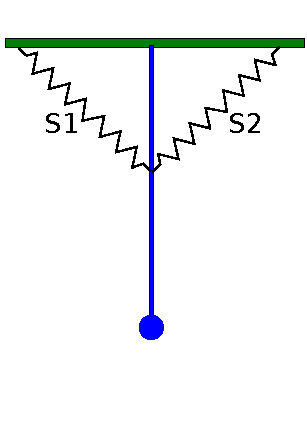
\includegraphics[width=.3\textwidth]{figures/pendulum_spring}
  \caption[pendulum with spring]{Pendulum model with two springs s1
    and s2}
  \label{fig:pendulum_spring}
\end{figure}


\subsection*{1.a Does the system have a stable limit cycle behavior?
  Describe and run an experiment to support your answer.}
\label{subsec:1.a}

\begin{figure}[H]
    \centering
    \begin{subfigure}[b]{0.5\textwidth}
        \centering
        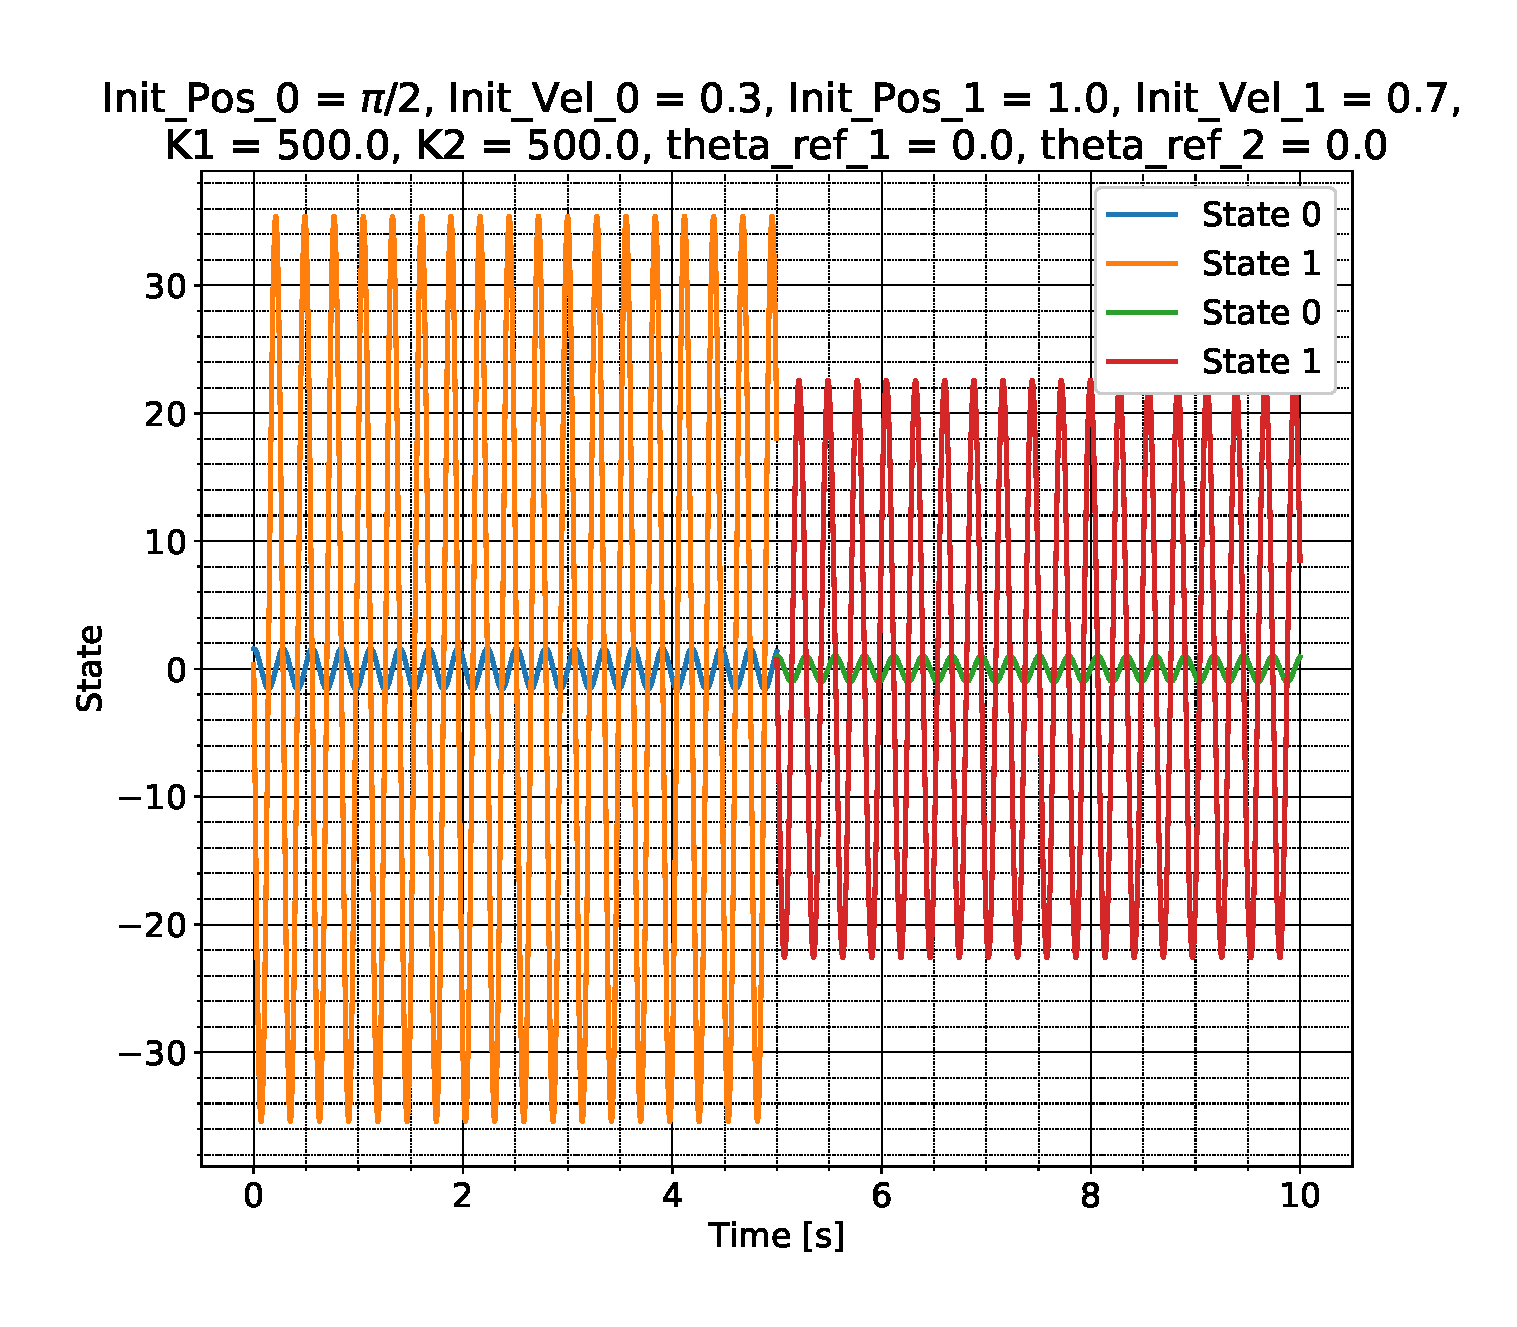
\includegraphics[height=3.2in]{New1.eps}
    \end{subfigure}%
    ~
    \begin{subfigure}[b]{0.5\textwidth}
        \centering
        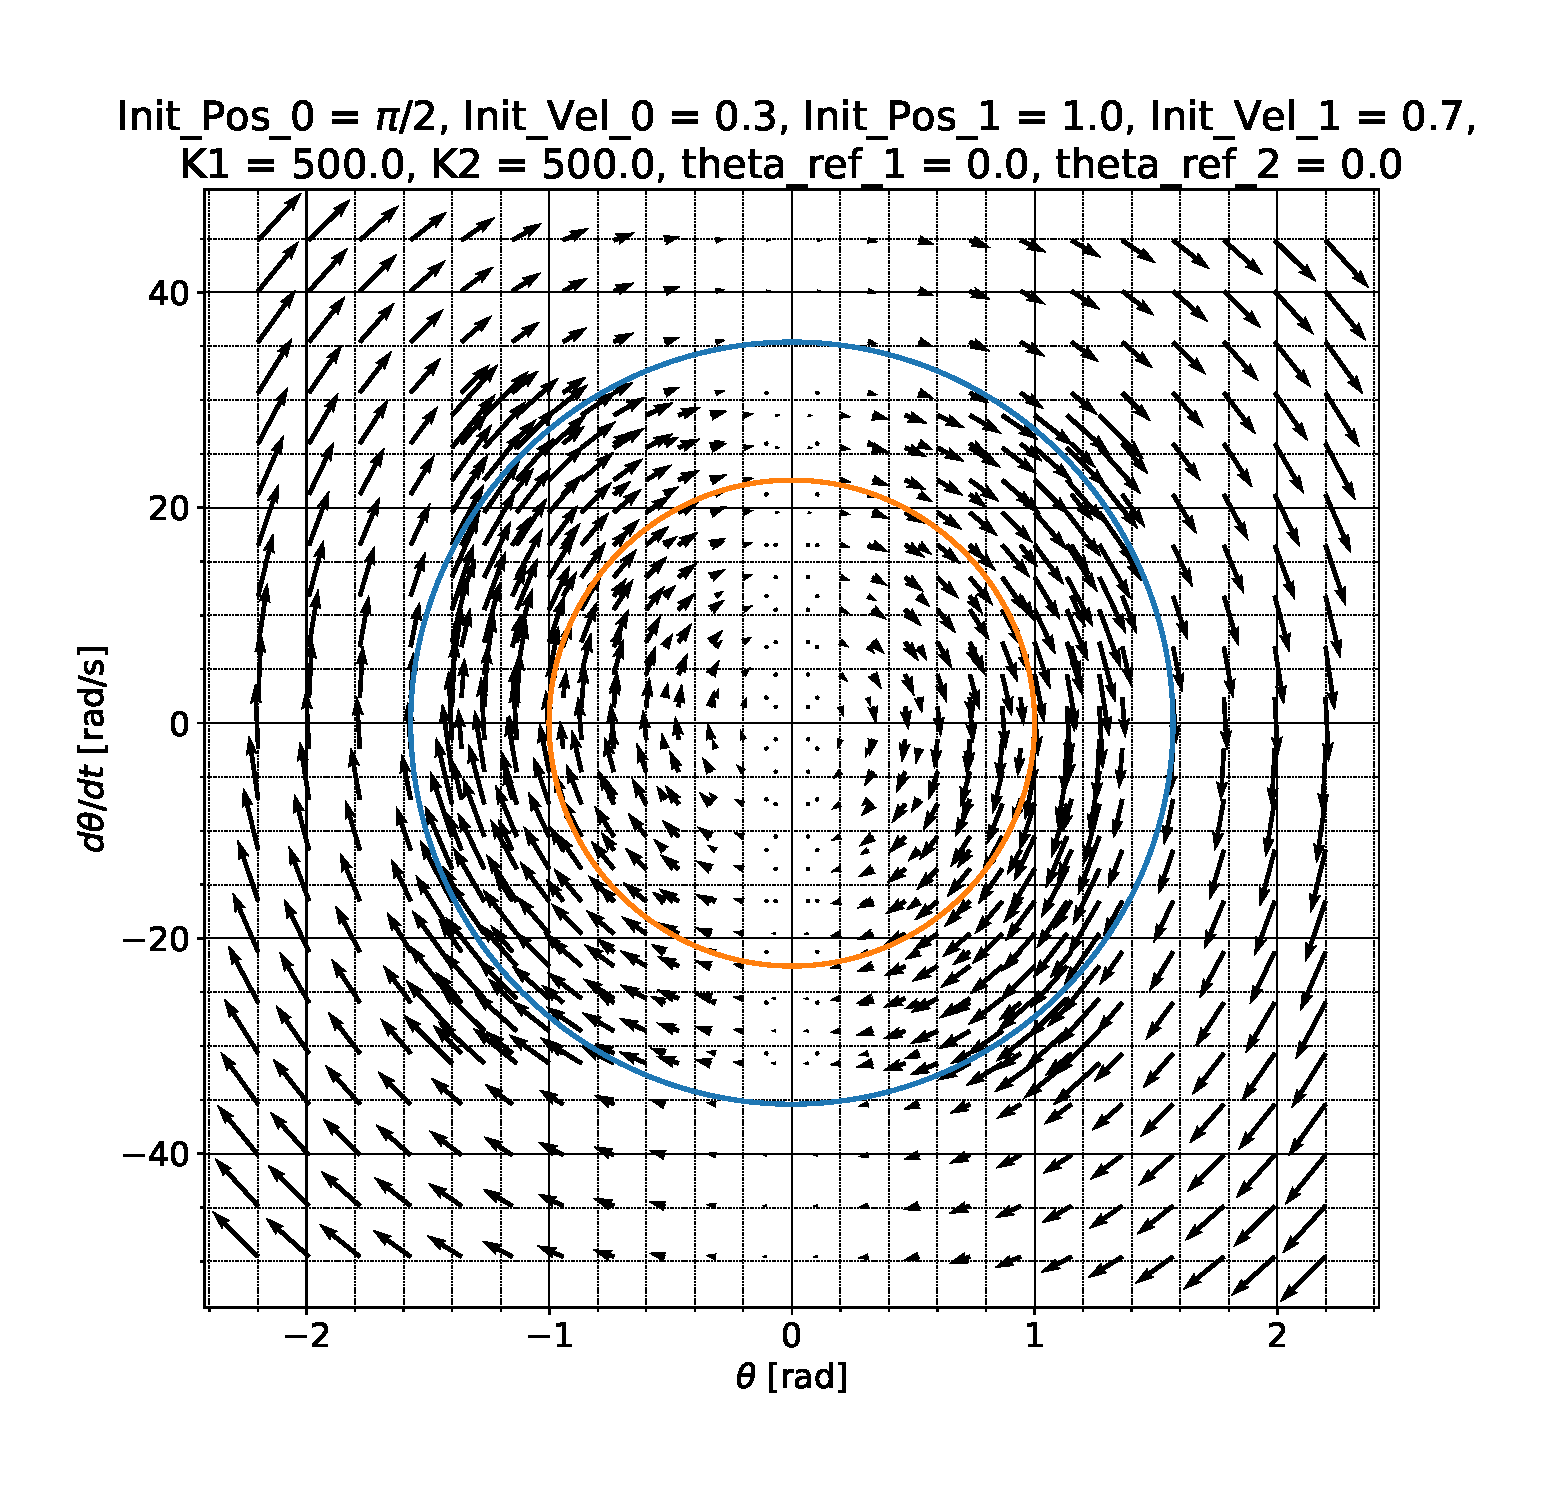
\includegraphics[height=3.2in]{New2.eps}
    \end{subfigure}
    \caption{Pendulum system, for which we induce a perturbation at half the time of the simulation. We start with a pendulum system with condition 0 (initial position = $\pi$/2, initial velocity = 0.3 rad/s) and we perturb it with what we called the condition 1 (position forced to 1.0 rad, velocity increased to 0.7 rad/s. Both springs otherwise share the same parameters in terms of reference angles and stiffness. The left part of the figure depicts the perturbation (Blue State 0: pendulum position before perturbation, orange State 1: pendulum velocity before perturbation, green State 0: pendulum position after perturbation, red State 1: pendulum velocity after perturbation) and the right part shows corresponding phase portraits (blue line corresponds to after perturbation). }
    \label{figure:1a}
\end{figure}

As we can see on Figure \ref{figure:1a}, where we disturb the system at mid-simulation time by forcing its position and velocity to new ones, the system will adapt to the new conditions - here, keeping the same angular velocity between conditions 0 and 1 wouldn't change anything to the phase portrait, it is the position that changes the system's behaviour. As we can see when comparing the left and right sides of Figure \ref{figure:1a}, the system oscillates perpetually since it is not dampen, and will simply adapt to the new position and velocities and oscillate continuously, without ever getting back to the same equilibrium ellipsoid on the phase portrait, which indicates that the system does not have a stable limit cycle behaviour.

\subsection*{1.b Explore the role of spring constant ($K$) and spring
  reference angle ($\theta_0$) in terms of range of motion, amplitude,
  ... \\ Support your responses with relevant plots }

\begin{figure}[H]
    \centering
    \begin{subfigure}[b]{0.5\textwidth}
        \centering
        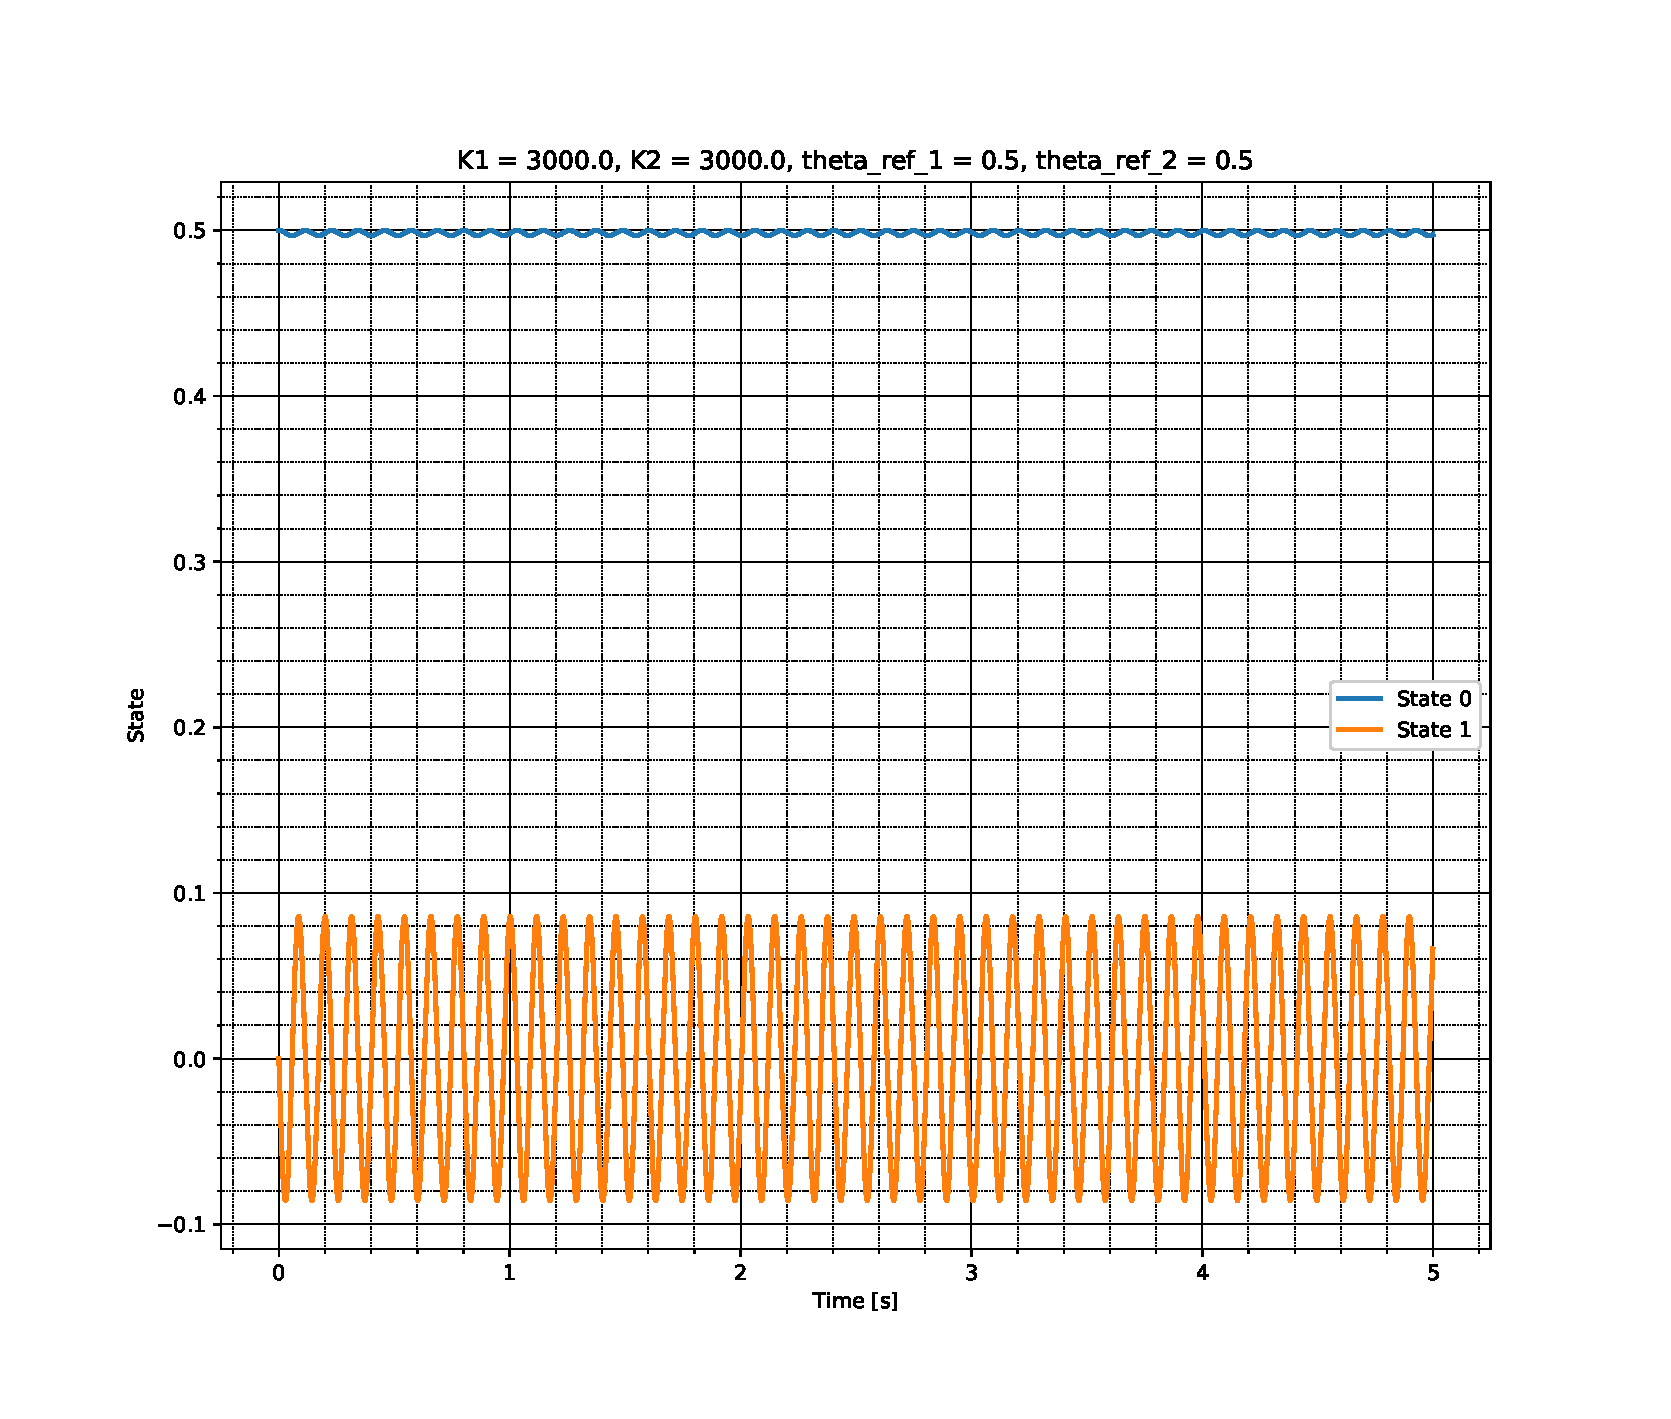
\includegraphics[height=2.8in]{1c_1a.eps}
    \end{subfigure}%
    ~
    \begin{subfigure}[b]{0.5\textwidth}
        \centering
        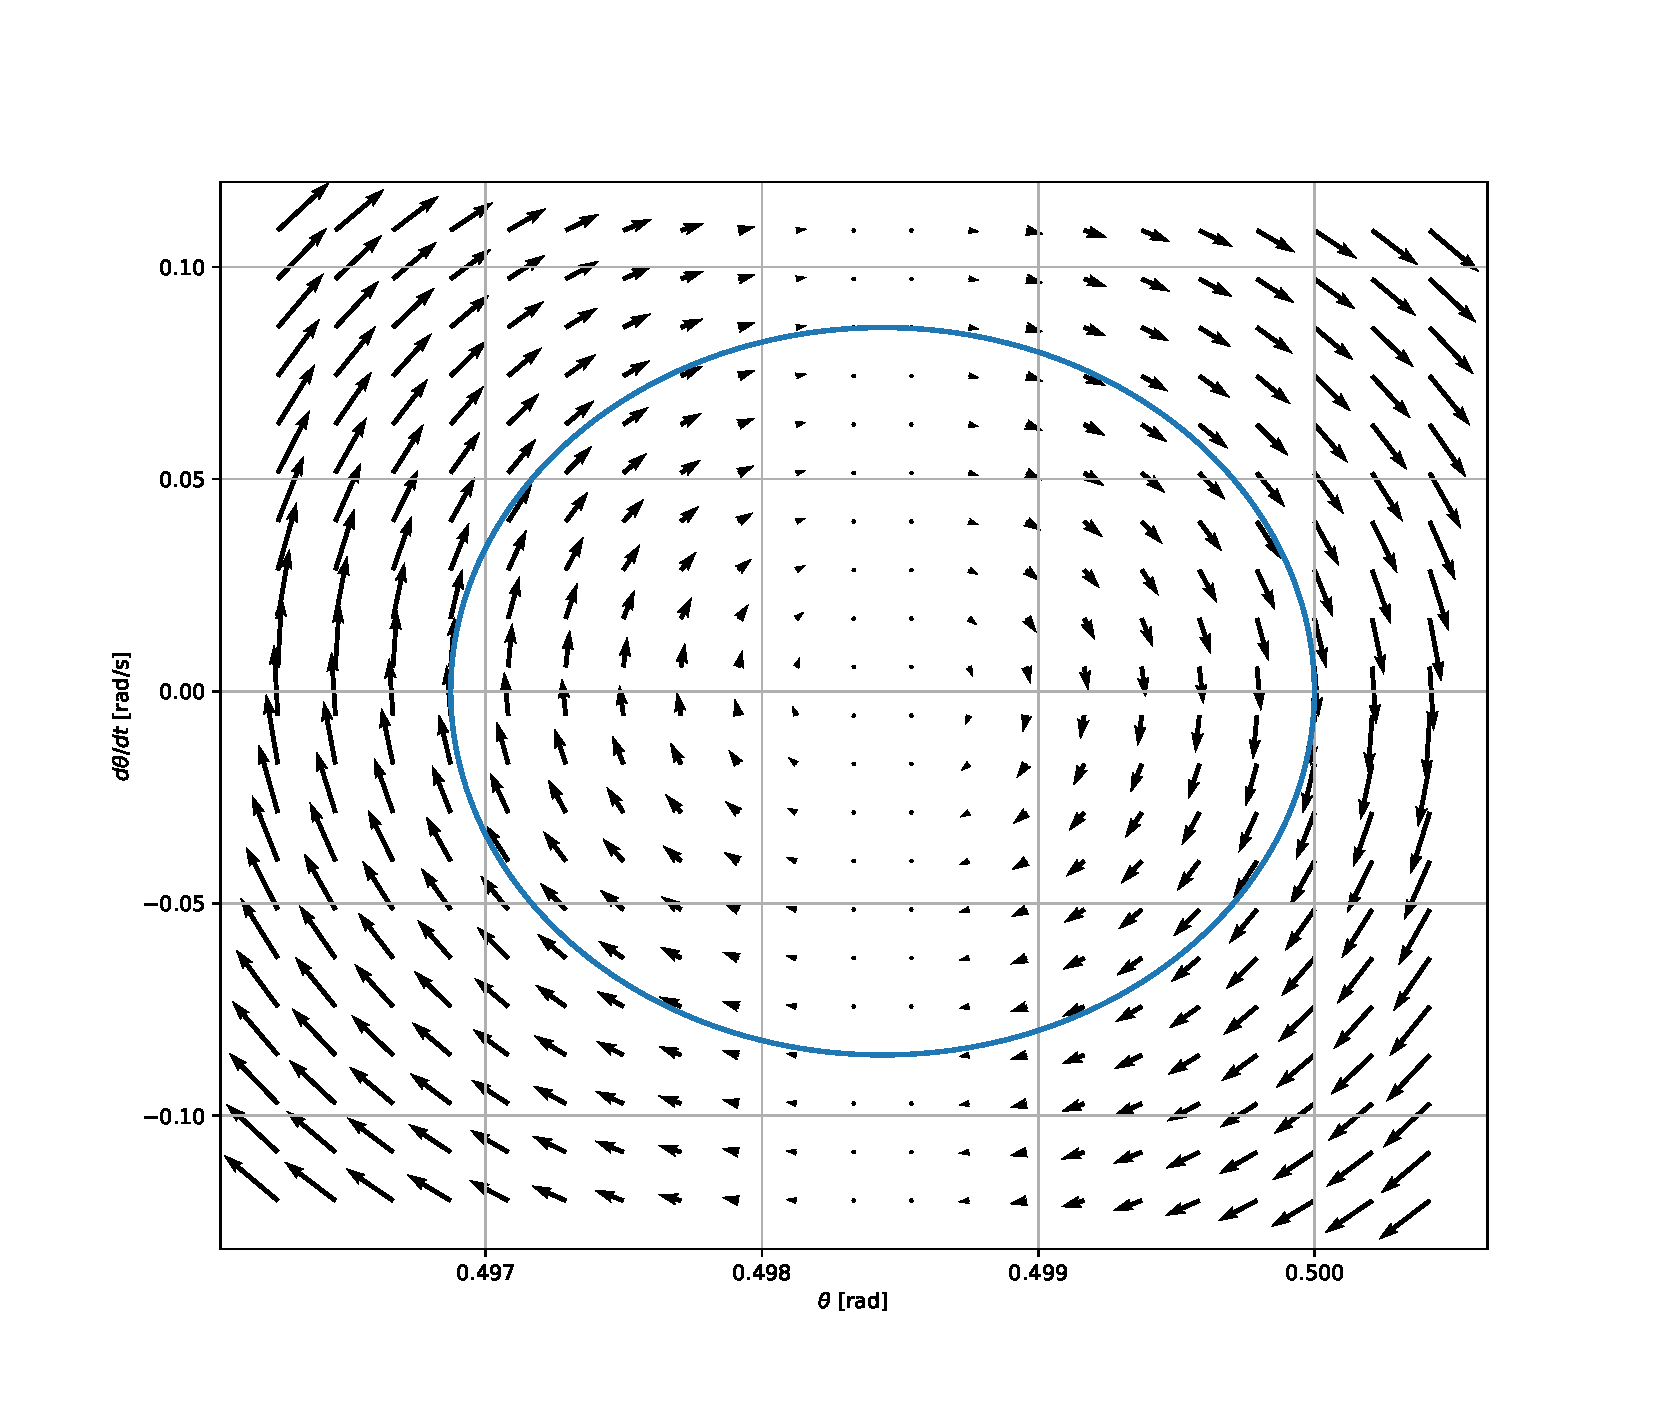
\includegraphics[height=2.8in]{1c_1b.eps}
    \end{subfigure}
    \caption{Angle (state 0) and angular velocity (state 1) as a function of time, with associated phase portrait. System of pendulum with 2 springs. Parameters written on top of the left figure.}
    \label{figure:1c1}
\end{figure}

For this first trial (see Figure \ref{figure:1c1}), the pendulum starts at the same angle $\theta=0.5$ corresponding to $\theta_{ref}$ of both springs, with two spring constants of $K=3000$. As we start at the resting position of the springs, the system should normally stay at rest. But as the gravity acts on the pendulum, we see low oscillations that tend to bring down the system toward $\theta=0$, which correspond to the minimal potential energy. However, since the springs are stiff (high spring constant), they maintain the system near their reference angle.

\begin{figure}[H]
    \centering
    \begin{subfigure}[b]{0.5\textwidth}
        \centering
        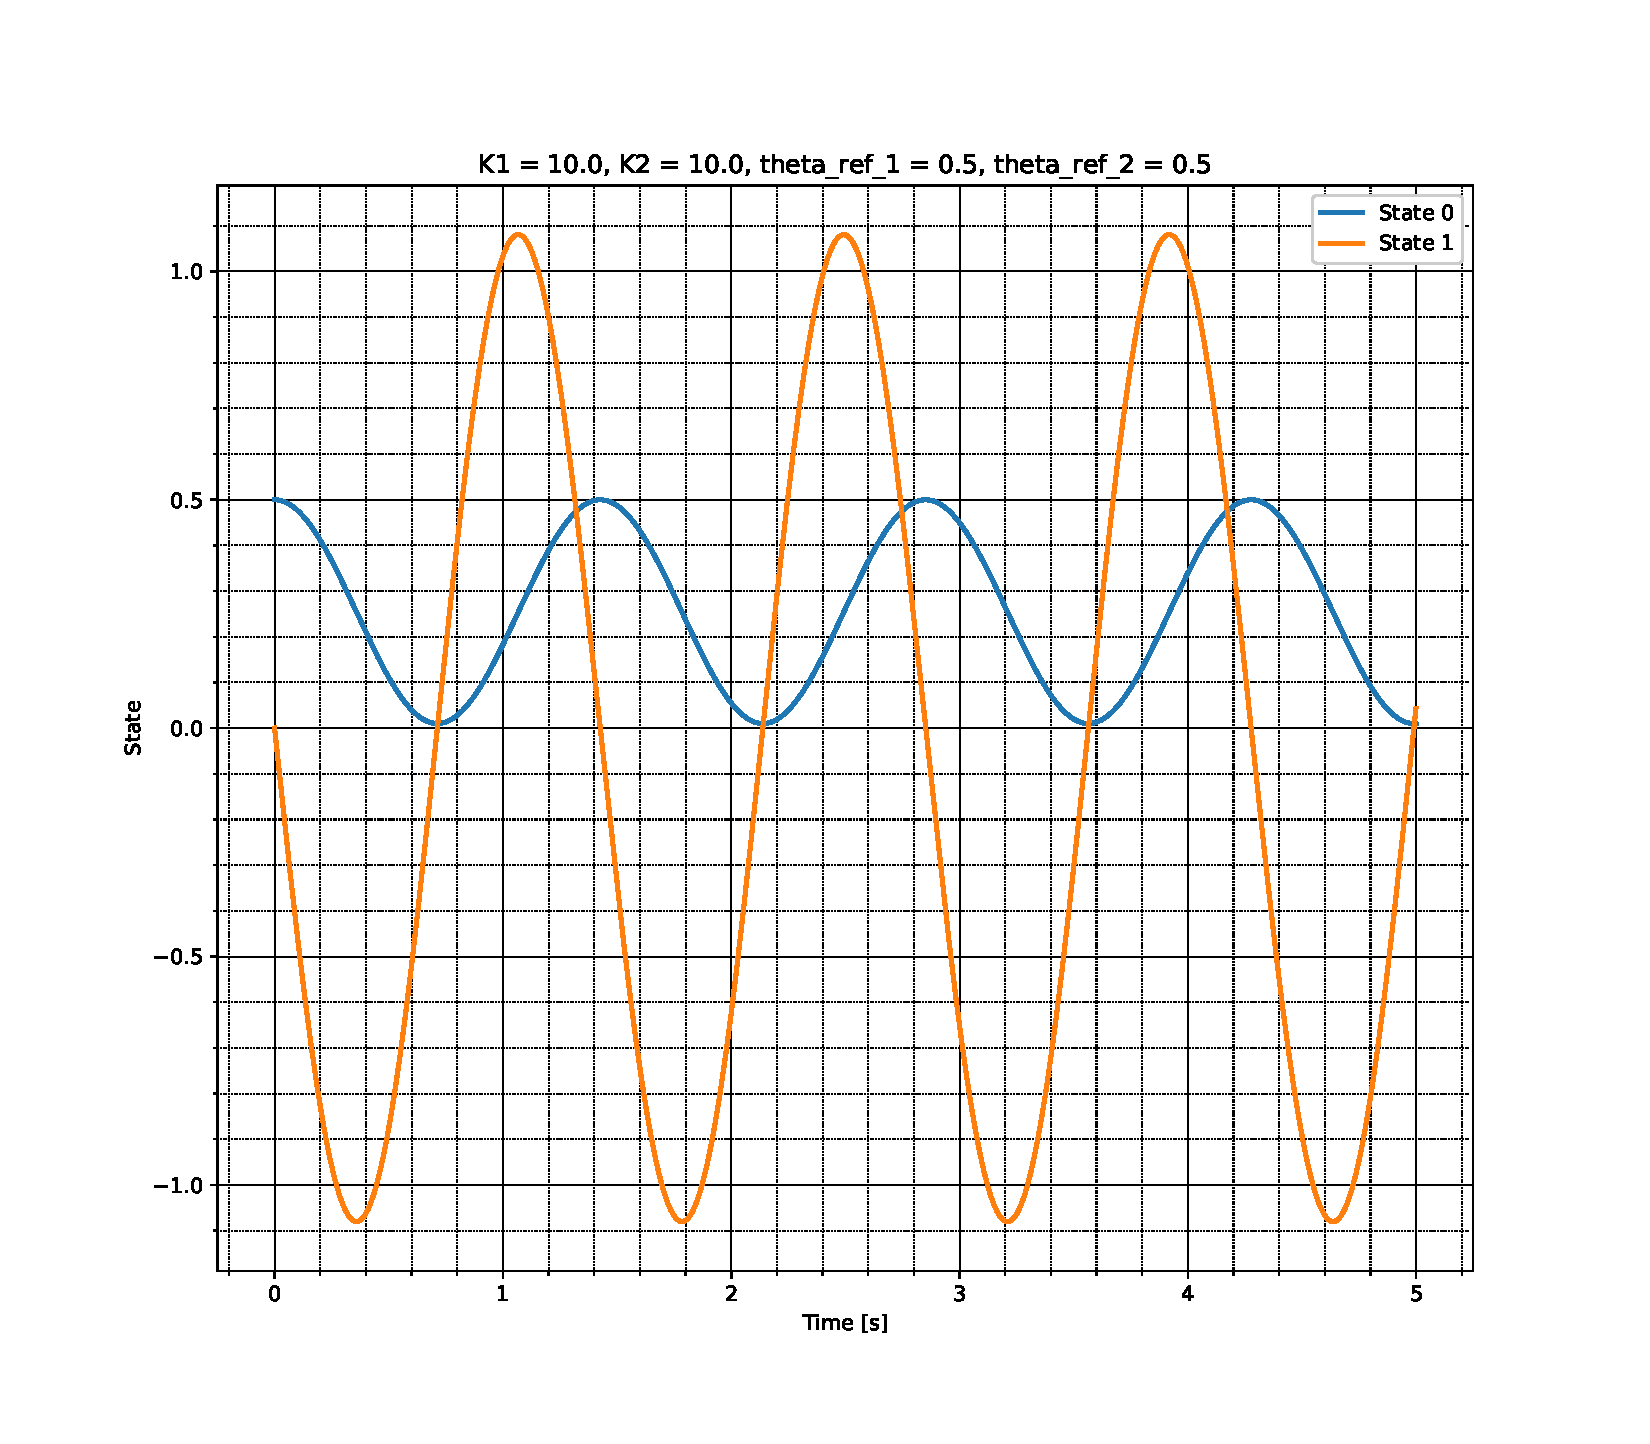
\includegraphics[height=2.8in]{1c_2a.eps}
    \end{subfigure}%
    ~
    \begin{subfigure}[b]{0.5\textwidth}
        \centering
        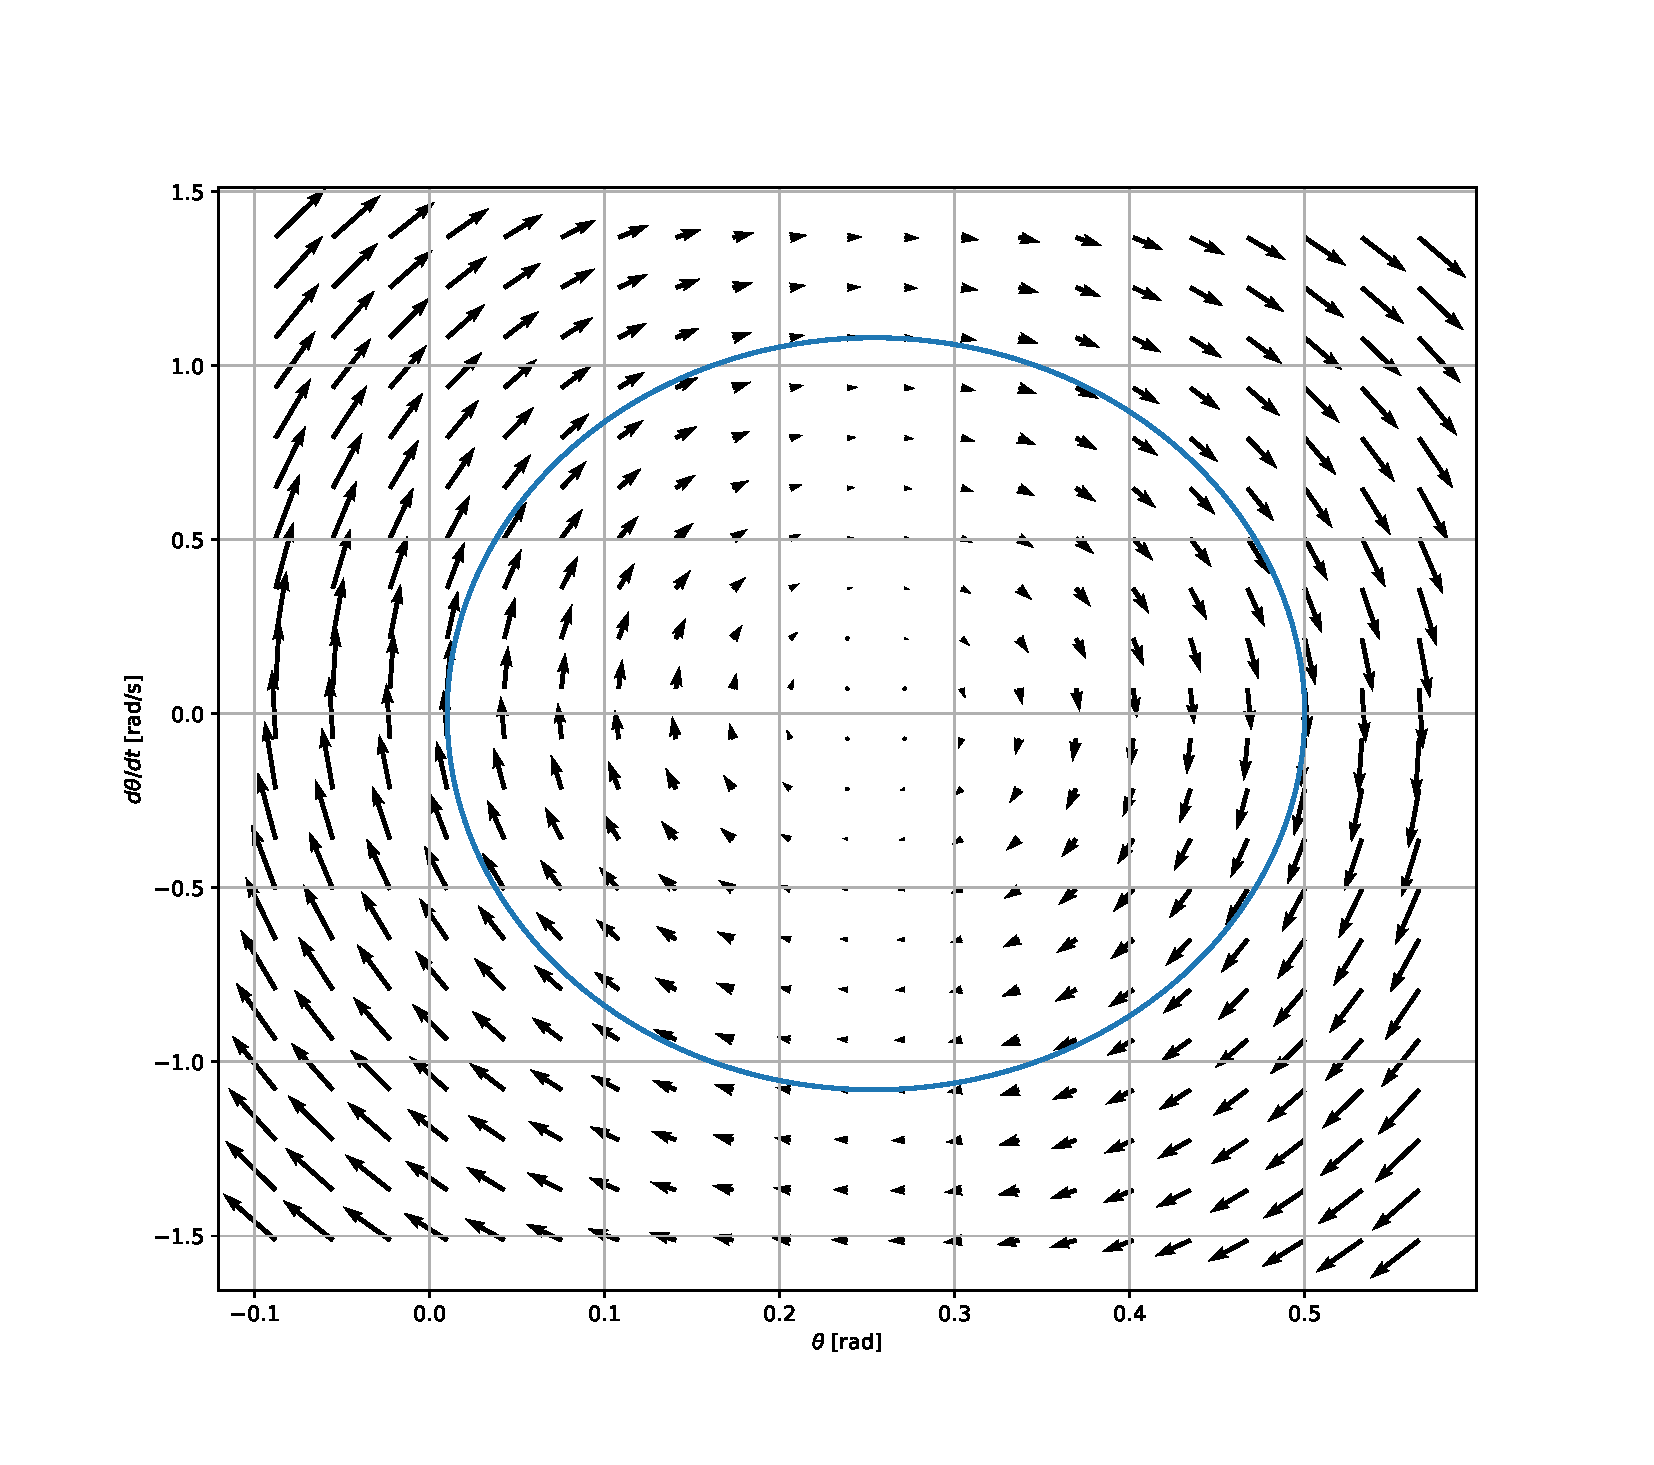
\includegraphics[height=2.8in]{1c_2b.eps}
    \end{subfigure}
    \caption{Angle (state 0) and angular velocity (state 1) as a function of time, with associated phase portrait. System of pendulum with 2 springs. Parameters written on top of the left figure.}
    \label{figure:1c2}
\end{figure}

For this second trial (see Figure \ref{figure:1c2}), we adjusted the system with low spring constants ($K=10$), but with similar initial conditions as for the first trial. We can see here much larger oscillations than in the first trial, with $\theta$ nearly reaching 0. Since the springs are less stiff, the contribution of the gravity is more apparent and have a greater impact on the system's equilibrium.

\begin{figure}[H]
    \centering
    \begin{subfigure}[b]{0.5\textwidth}
        \centering
        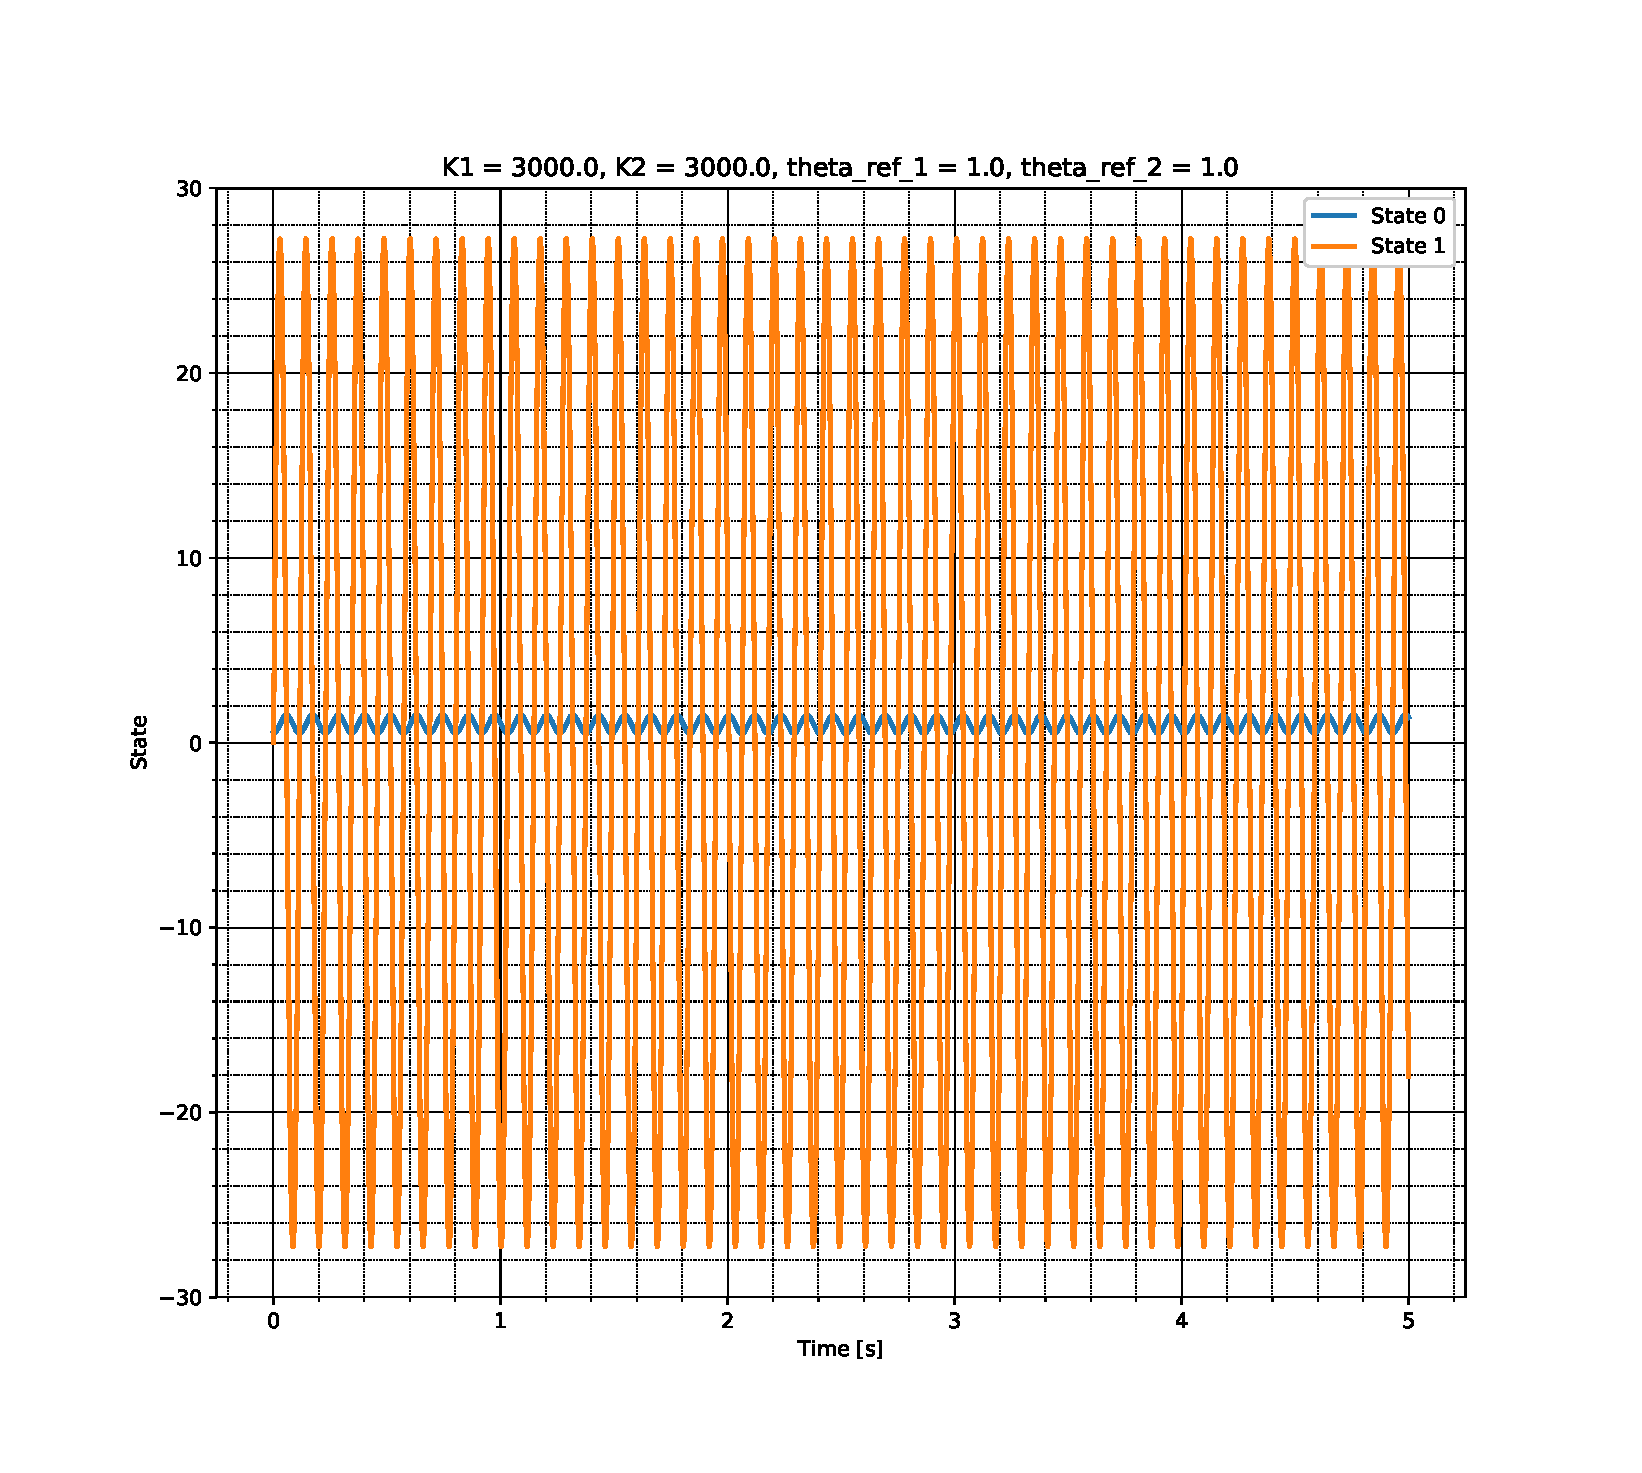
\includegraphics[height=2.8in]{1c_3a.eps}
    \end{subfigure}%
    ~
    \begin{subfigure}[b]{0.5\textwidth}
        \centering
        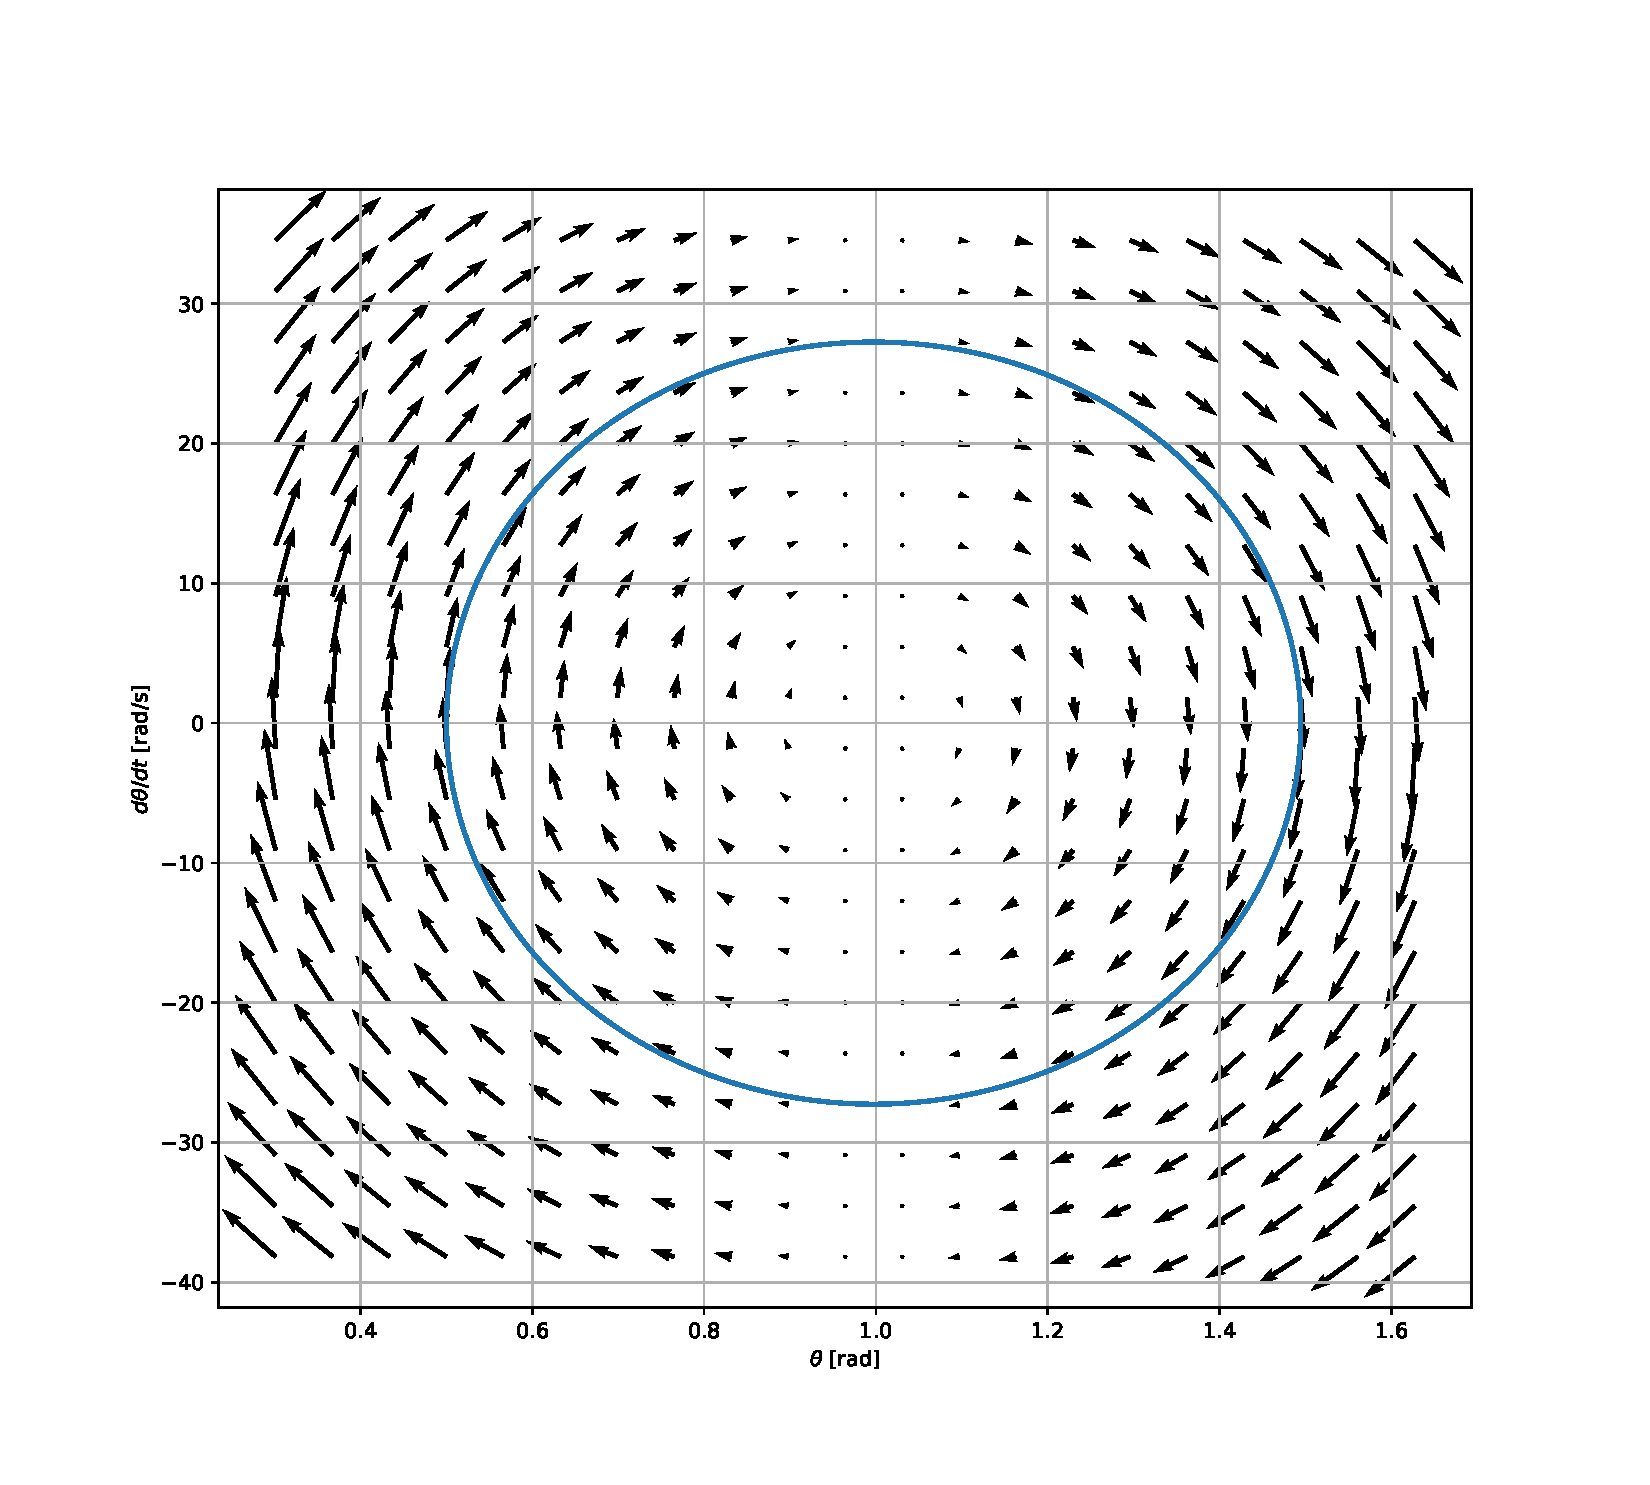
\includegraphics[height=2.8in]{1c_3b.eps}
    \end{subfigure}
    \caption{Angle (state 0) and angular velocity (state 1) as a function of time, with associated phase portrait. System of pendulum with 2 springs. Parameters written on top of the left figure.}
    \label{figure:1c3}
\end{figure}

Finally, we start the position of the pendulum at $\theta=0.5$, set the reference angle of both springs to $\theta_{ref}=1.0$, and both springs to a spring coefficient of $K=3000$. On Figure \ref{figure:1c3}, especially in the phase portrait, we observe that the initial position in this context will define the amplitude, and the reference angle acts as as an equilibrium point around which the pendulum oscillates.

To conclude, we observe that the spring constant $K$ has a role to play in characterising the spring's influence on the whole system in terms of total equilibrium angle and oscillatory period, and that $\theta_{ref}$, the contribution of each spring to the system's equilibrium, is depending on the $K$'s. In other words, we can say that the if the stiffness of one spring is increased, the equilibrium point of the pendulum will be more influenced by this spring's reference angle. If the stiffness of one spring is much larger than the other, it will pull the equilibrium $\theta$ towards its $\theta_{ref}$.

\subsection*{1.c Explain the behavior of the model when you have
  different spring constants ($K$) and spring reference angles
  ($\theta_{ref}$). Support your responses with relevant plots}

\begin{figure}[H]
    \centering
    \begin{subfigure}[b]{0.5\textwidth}
        \centering
        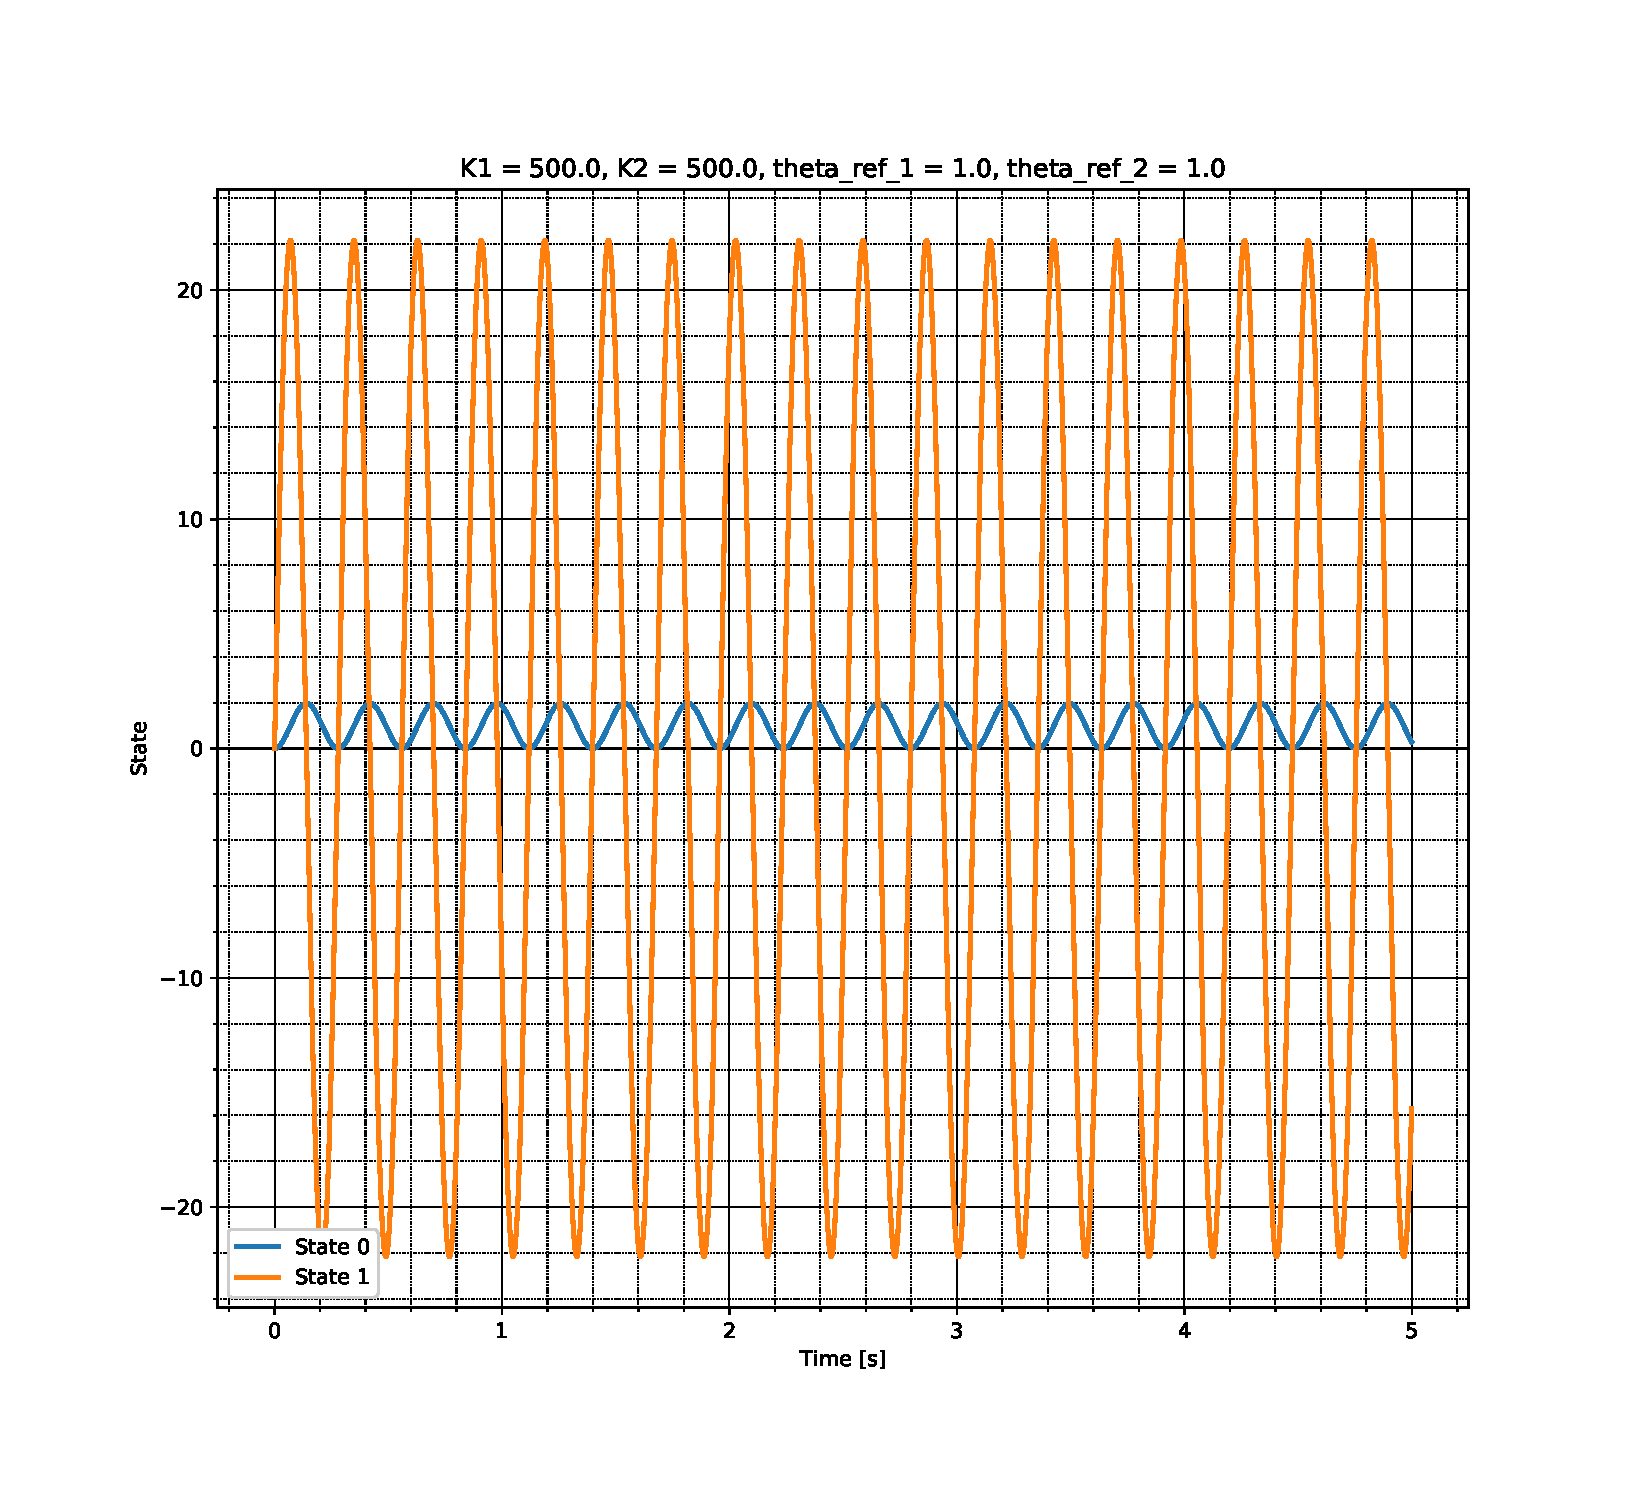
\includegraphics[height=3.5in]{1b_1.eps}
        \caption{}
    \end{subfigure}%
    ~
    \begin{subfigure}[b]{0.5\textwidth}
        \centering
        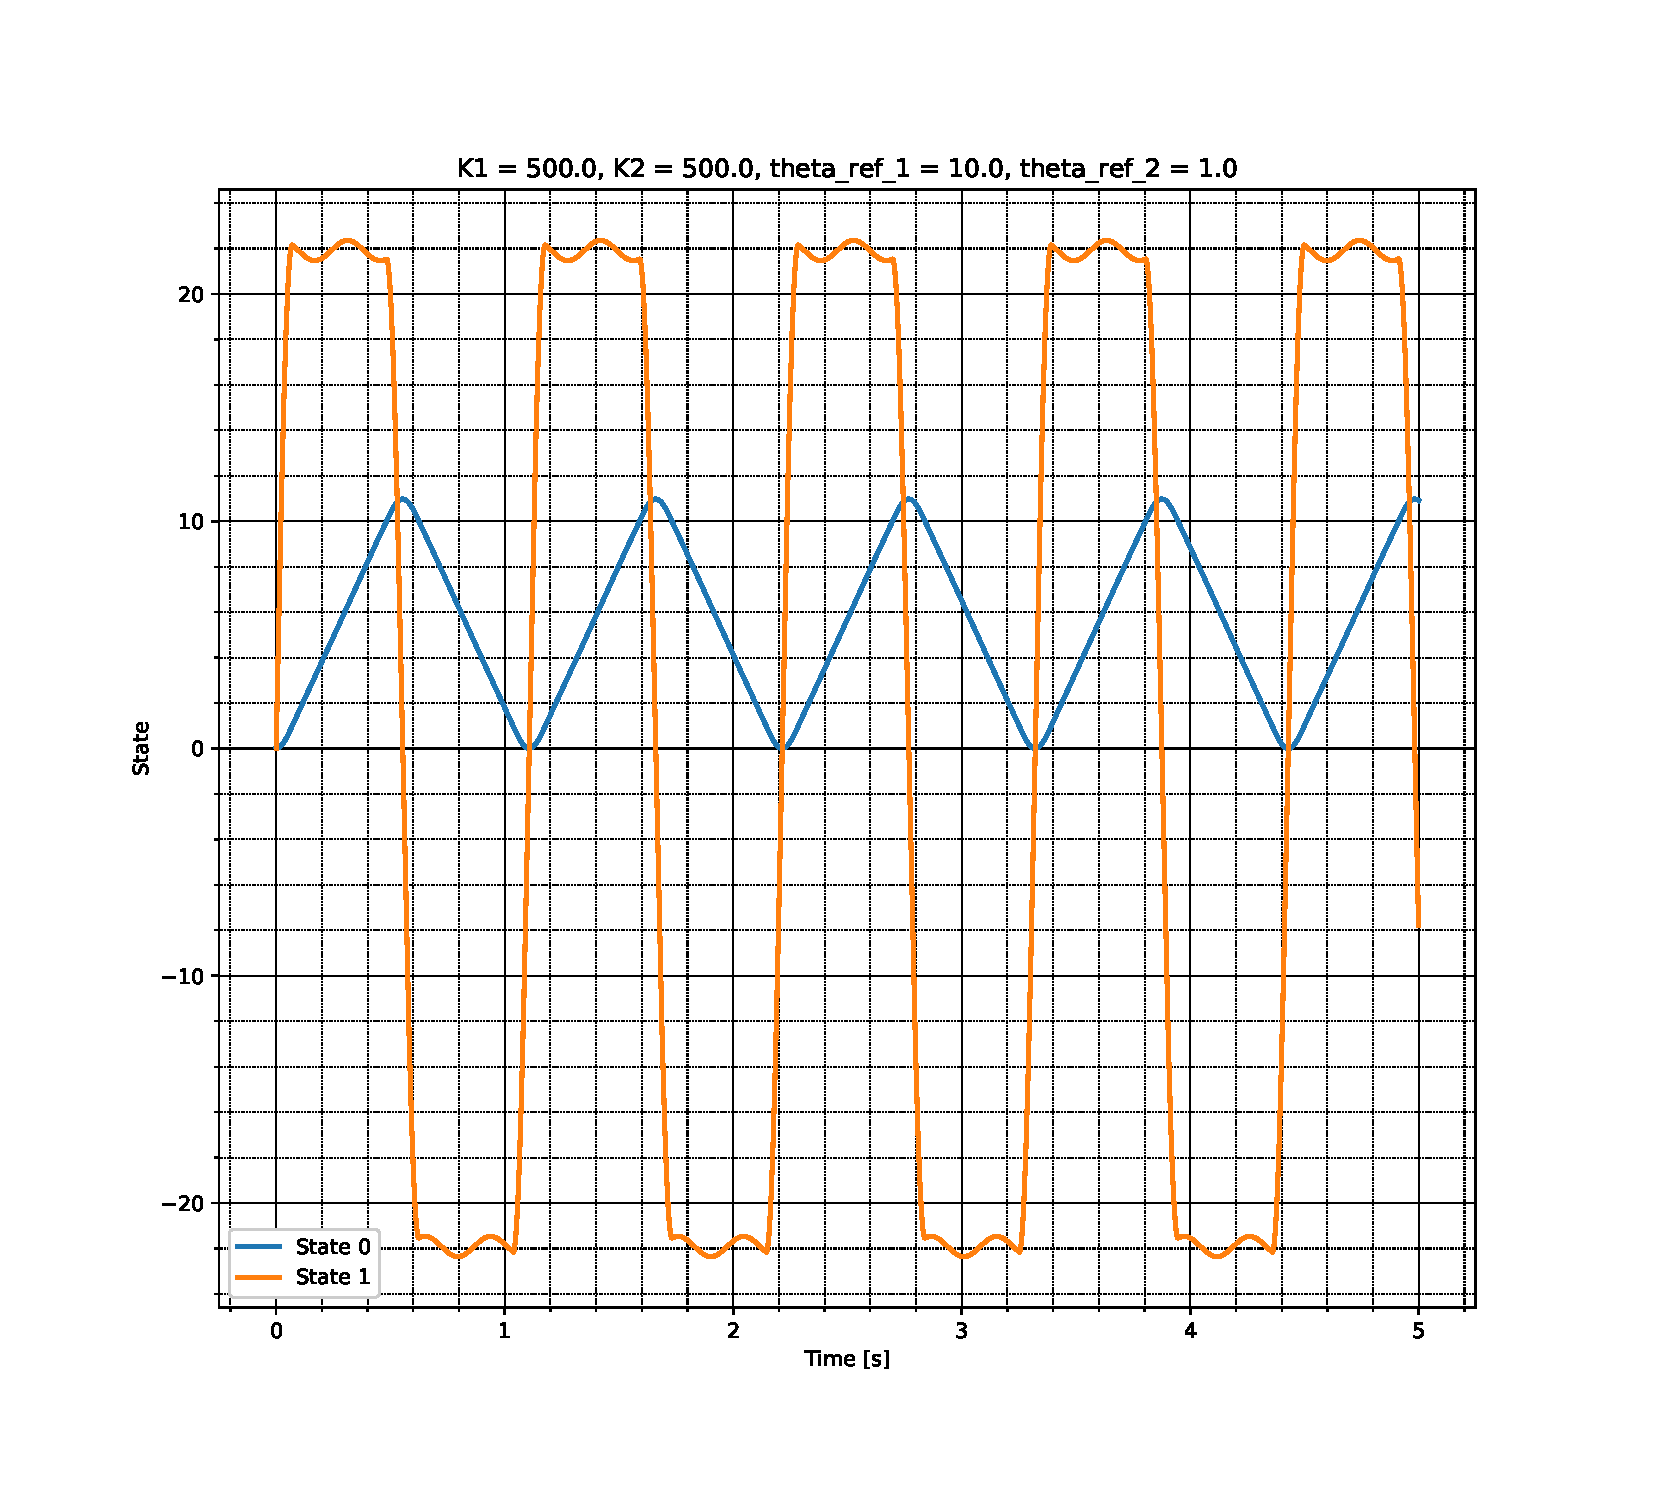
\includegraphics[height=3.5in]{1b_2.eps}
        \caption{}
    \end{subfigure}
    \bigskip
    \begin{subfigure}[b]{0.5\textwidth}
        \centering
        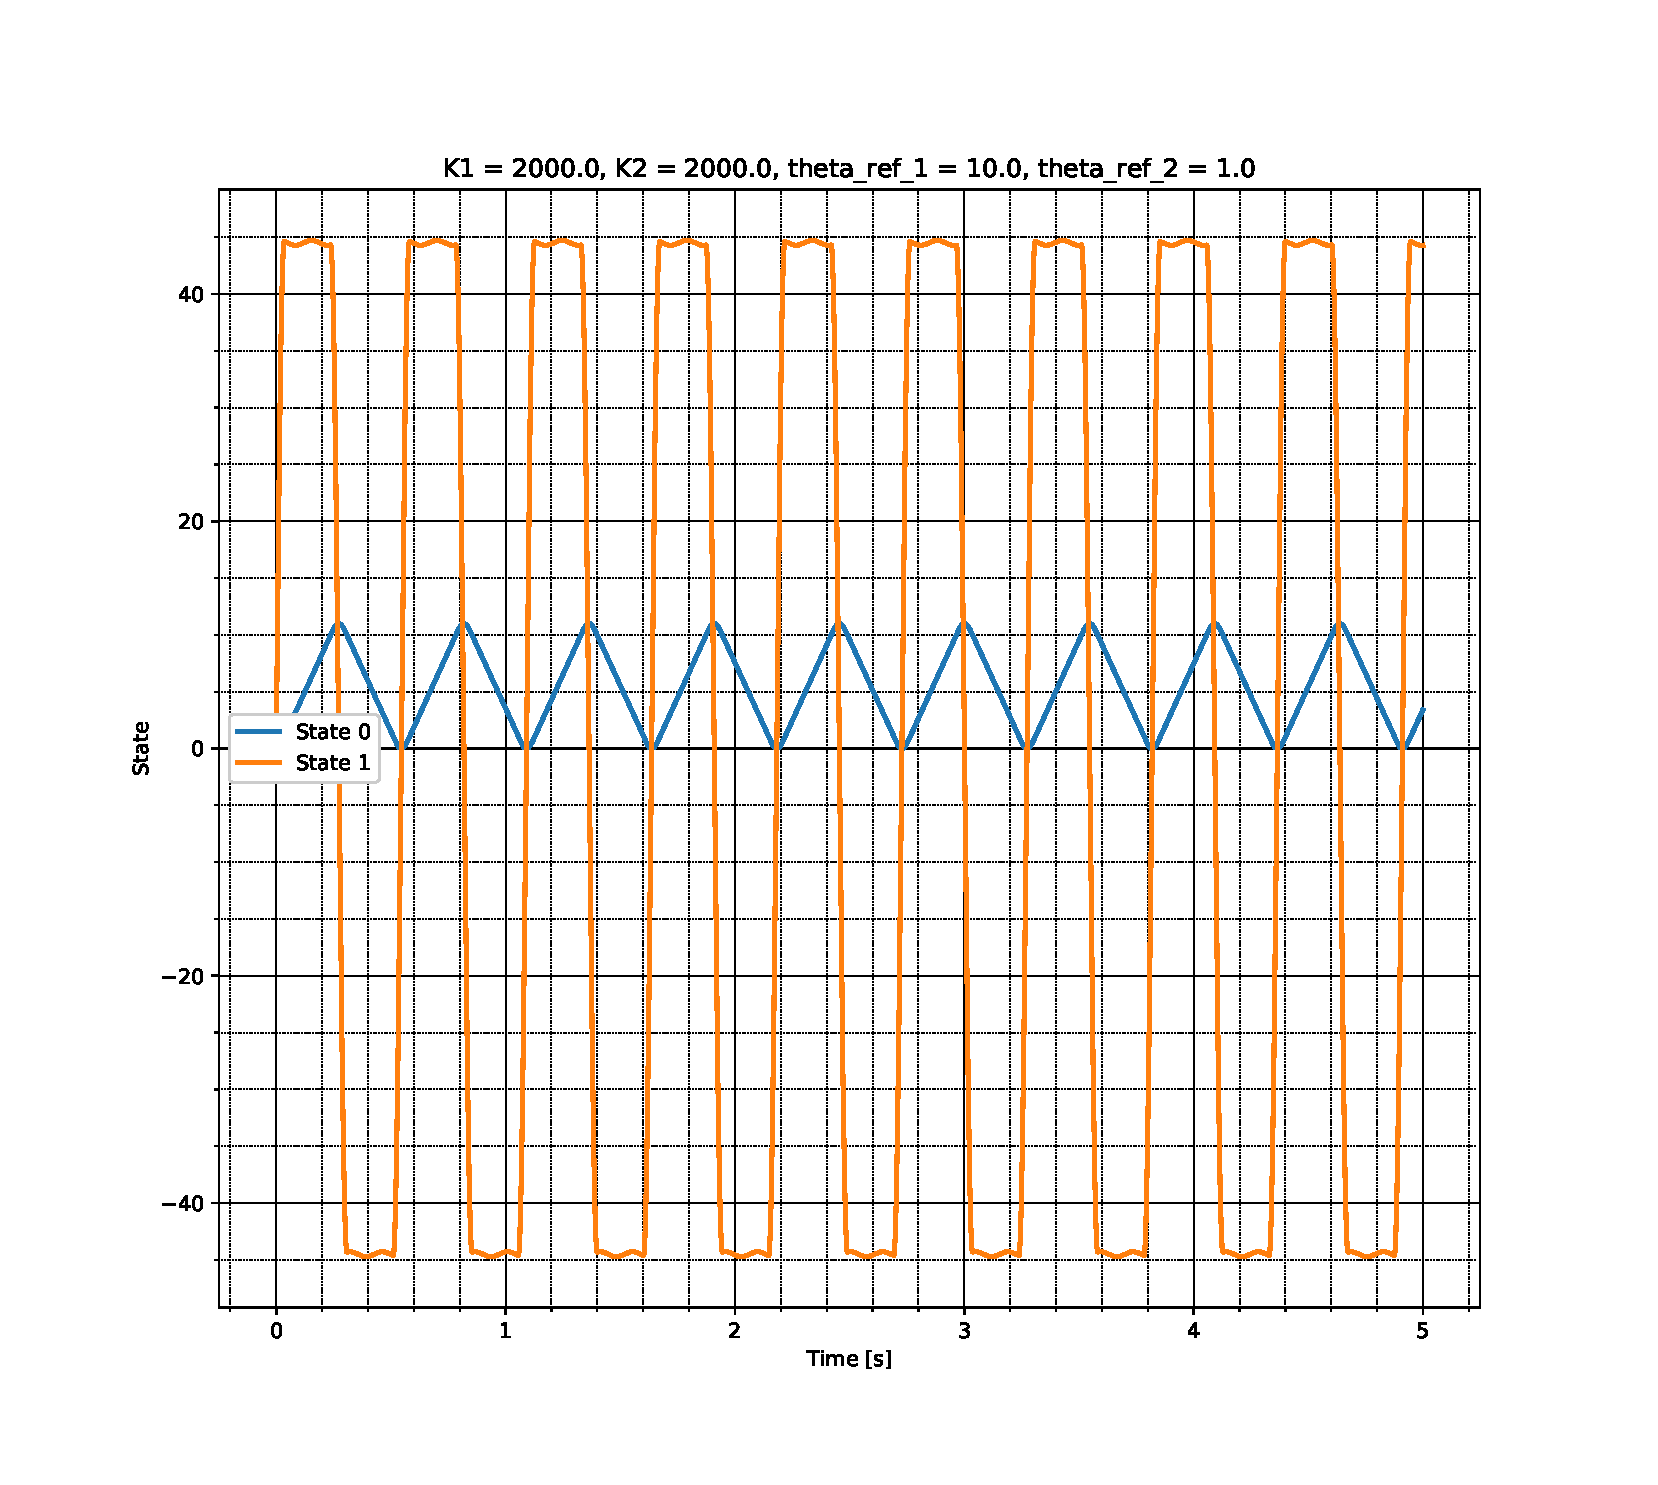
\includegraphics[height=3.5in]{1b_3.eps}
        \caption{}
    \end{subfigure}%
    ~
    \begin{subfigure}[b]{0.5\textwidth}
        \centering
        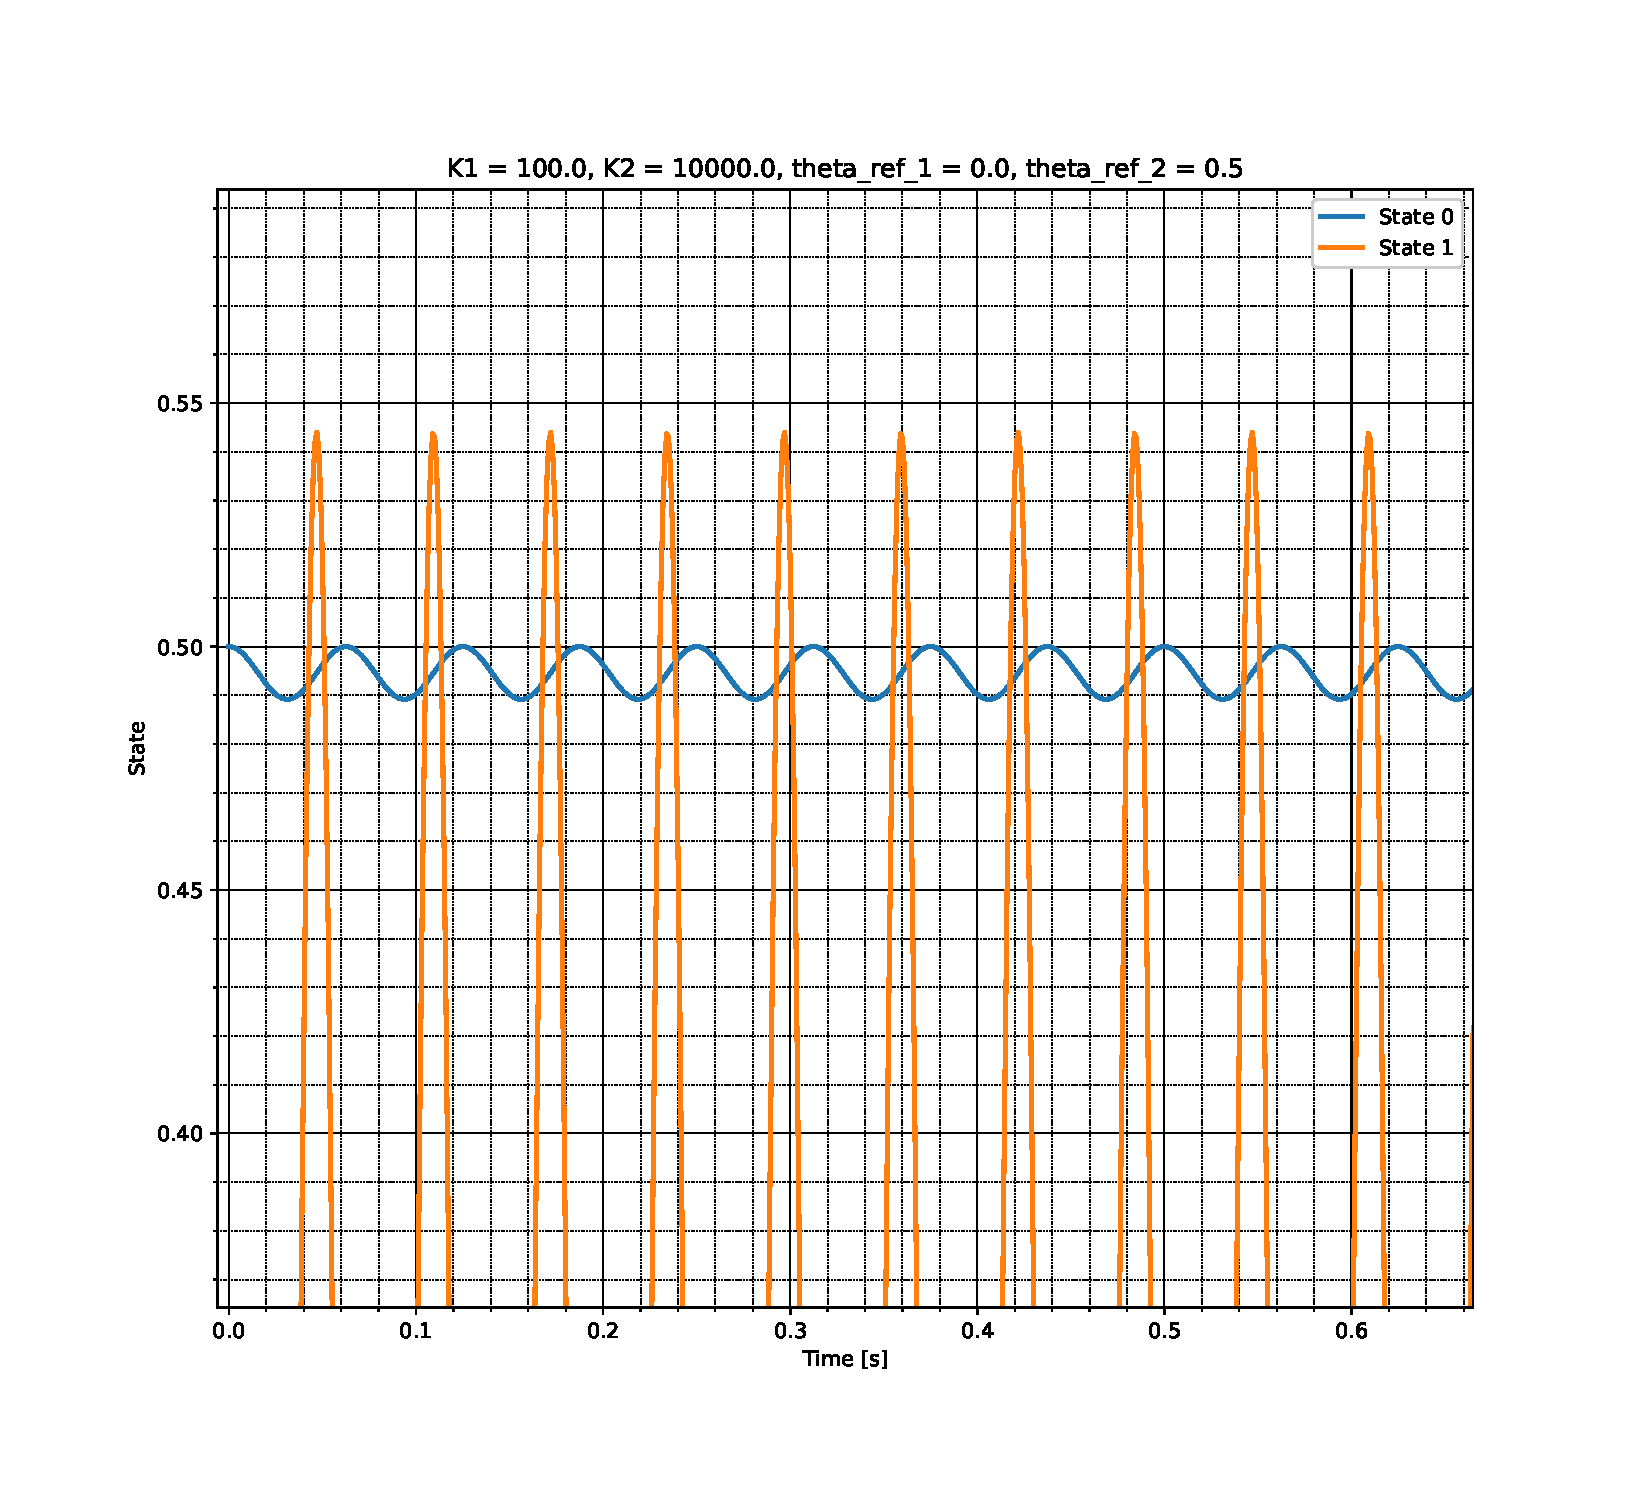
\includegraphics[height=3.5in]{1b_4.eps}
        \caption{}
    \end{subfigure}
    \caption{Angle (state 0) and angular velocity (state 1) as a function of time.  System of pendulum with 2 springs. Different plot with varying spring constants and $\theta_{ref}$. Initial conditions for all simulations: position = velocity = 0.}
    \label{figure:1b}
\end{figure}

To address this question, we ran 4 simulations, for which the initial conditions of the system were always 0 for position and velocities: we begin with identical conditions for both springs ($K1 = K2 = 500$ [N/m], $\theta_{ref1,2}=1.0$ rad) - see Figure \ref{figure:1b}a. We observe that the system oscillates regularly around an equilibrium position of 1.0, corresponding to the weighted sum of both $\theta_{ref}$'s.

Then we set $\theta_{ref}$ to 10.0 radians (see Figure \ref{figure:1b}b). Regarding the angular velocity, we can see that the oscillatory behavior is composed: as the spring with $\theta_{ref}$ = 10 tries and pulls the pendulum towards this position (large oscillations in velocity), the spring with $\theta_{ref}$ = 1 will try to bring it back to $\theta$ = 1, which will cause the small oscillations that we observe within the larger ones in the velocity line. Of course, the total system oscillates around 5.5 rad, which is the weighted sum of the two $\theta_{refs}$. Then, increasing the spring constant (see Figure \ref{figure:1b}c) returns bigger amplitude in angular velocity and a higher oscillatory period, but the equilibrium position is the same as before, and so is the oscillatory behavior in the velocity. Finally, with different spring constants and reference angles (see Figure \ref{figure:1b}d), as hypothesized in point 1.b, the system oscillates around a weighted mean of the two $\theta_{refs}$ ($\theta_{ref1} = 0.0$, $\theta_{ref2} = 0.5$ [rad]). Since one of the spring constant is much higher than the other ($K1 = 100.0$, $K2 = 10000.0$ [N/m]), the corresponding $\theta_{ref2}$ will have more influence on the system's equilibrium. The velocity oscillations were big compared to the positional oscillations since one of the spring constant is a hundredth of the other, so we had to zoom in to observe the equilibrium position.

\subsection*{Explore the pendulum model with two antagonist spring and damper elements}
Over time muscles lose energy while doing work. In order to account
for this property, let us now add a damper in parallel to the spring
model. Use equation \ref{eqn:damper} to develop the damper model.

\textit{\textbf{Note} : Like the previous springs, dampers can only
  produce force in one-direction.  That is, they can only apply a
  damping force in the pulling direction and apply a zero force when
  compressed. You need to accommodate for this condition for dampers B1
  and B2 in the equation shown below}

Again use \fileref{exercise1.py}, \fileref{lab4\_pendulum.py} and
\fileref{SystemParameters.py} files to complete the exercise. The
setup for the pendulum model with a pair of antagonist spring and
dampers in parallel is as shown in figure
\ref{fig:pendulum_spring_damper}.


\begin{equation}
  \label{eqn:damper}
  F_{B} = B*(\dot{\theta})
\end{equation}

Where,
\begin{itemize}
\item $F_{B}$ : Torsional Damper force
\item $B$ : Damping Constant
\item $\dot{\theta}$ : pendulum angular velocity
\end{itemize}


\begin{figure}[H]
  \centering
  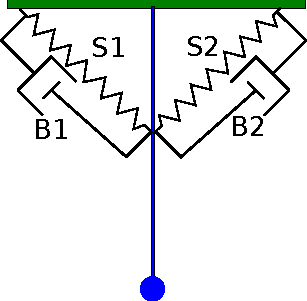
\includegraphics[width=.3\textwidth]{figures/pendulum_spring_damper}
  \caption[pendulum with spring]{Pendulum model with two springs S1
    and S2 and two dampers B1 and B2}
  \label{fig:pendulum_spring_damper}
\end{figure}


\subsection*{1.d How does the behavior now change compared to
  1.a. Briefly explain and support your responses with relevant plots}

\begin{figure}[H]
    \centering
    \begin{subfigure}[b]{0.5\textwidth}
        \centering
        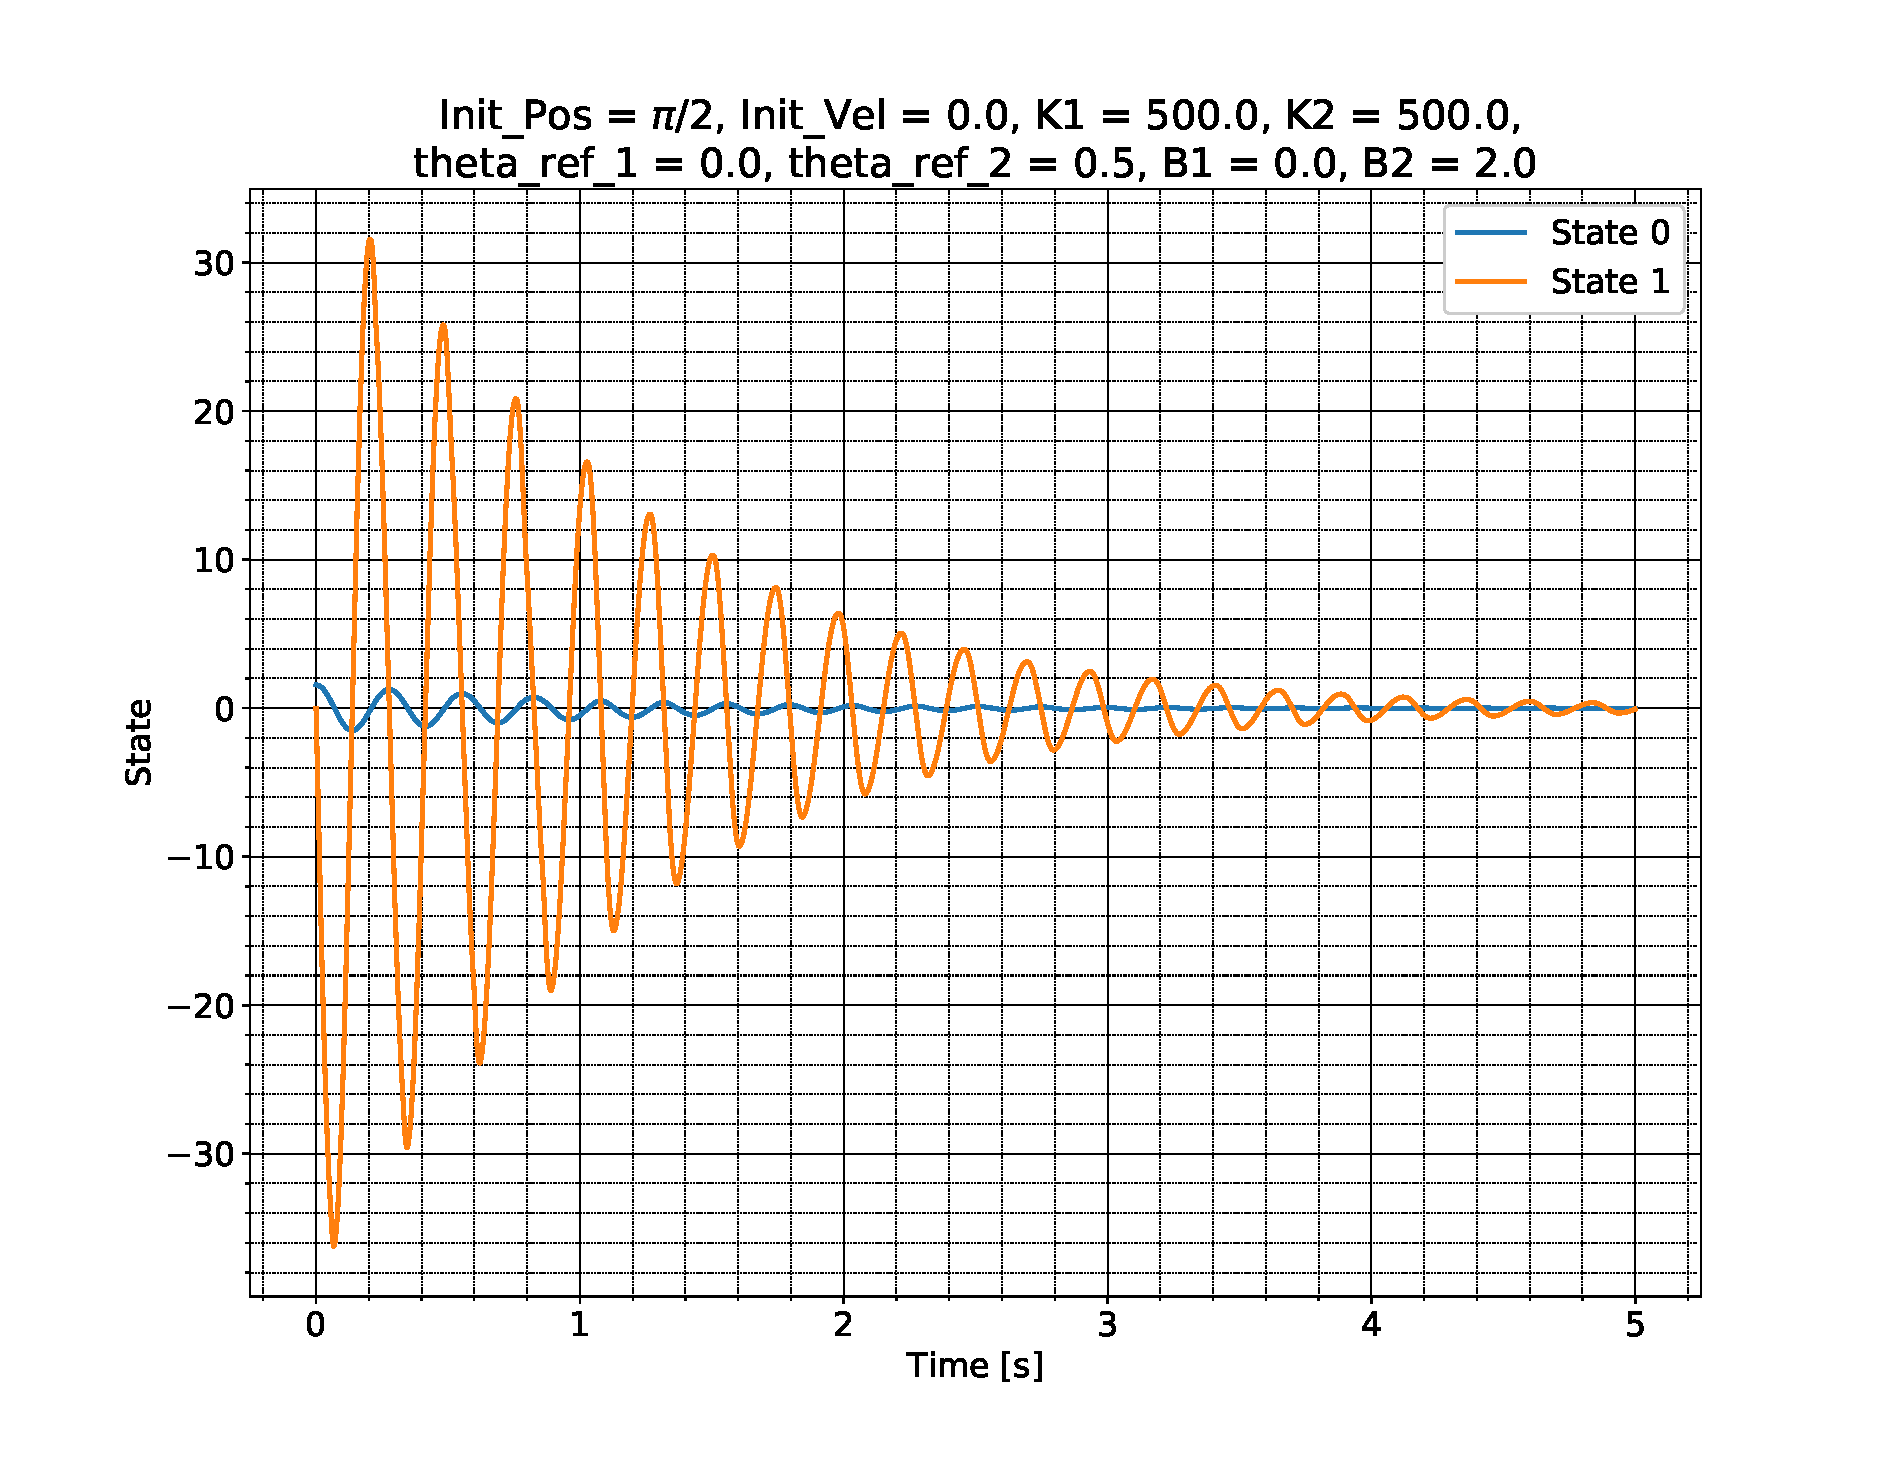
\includegraphics[height=2.8in]{1d_1.eps}
    \end{subfigure}%
    ~
    \begin{subfigure}[b]{0.5\textwidth}
        \centering
        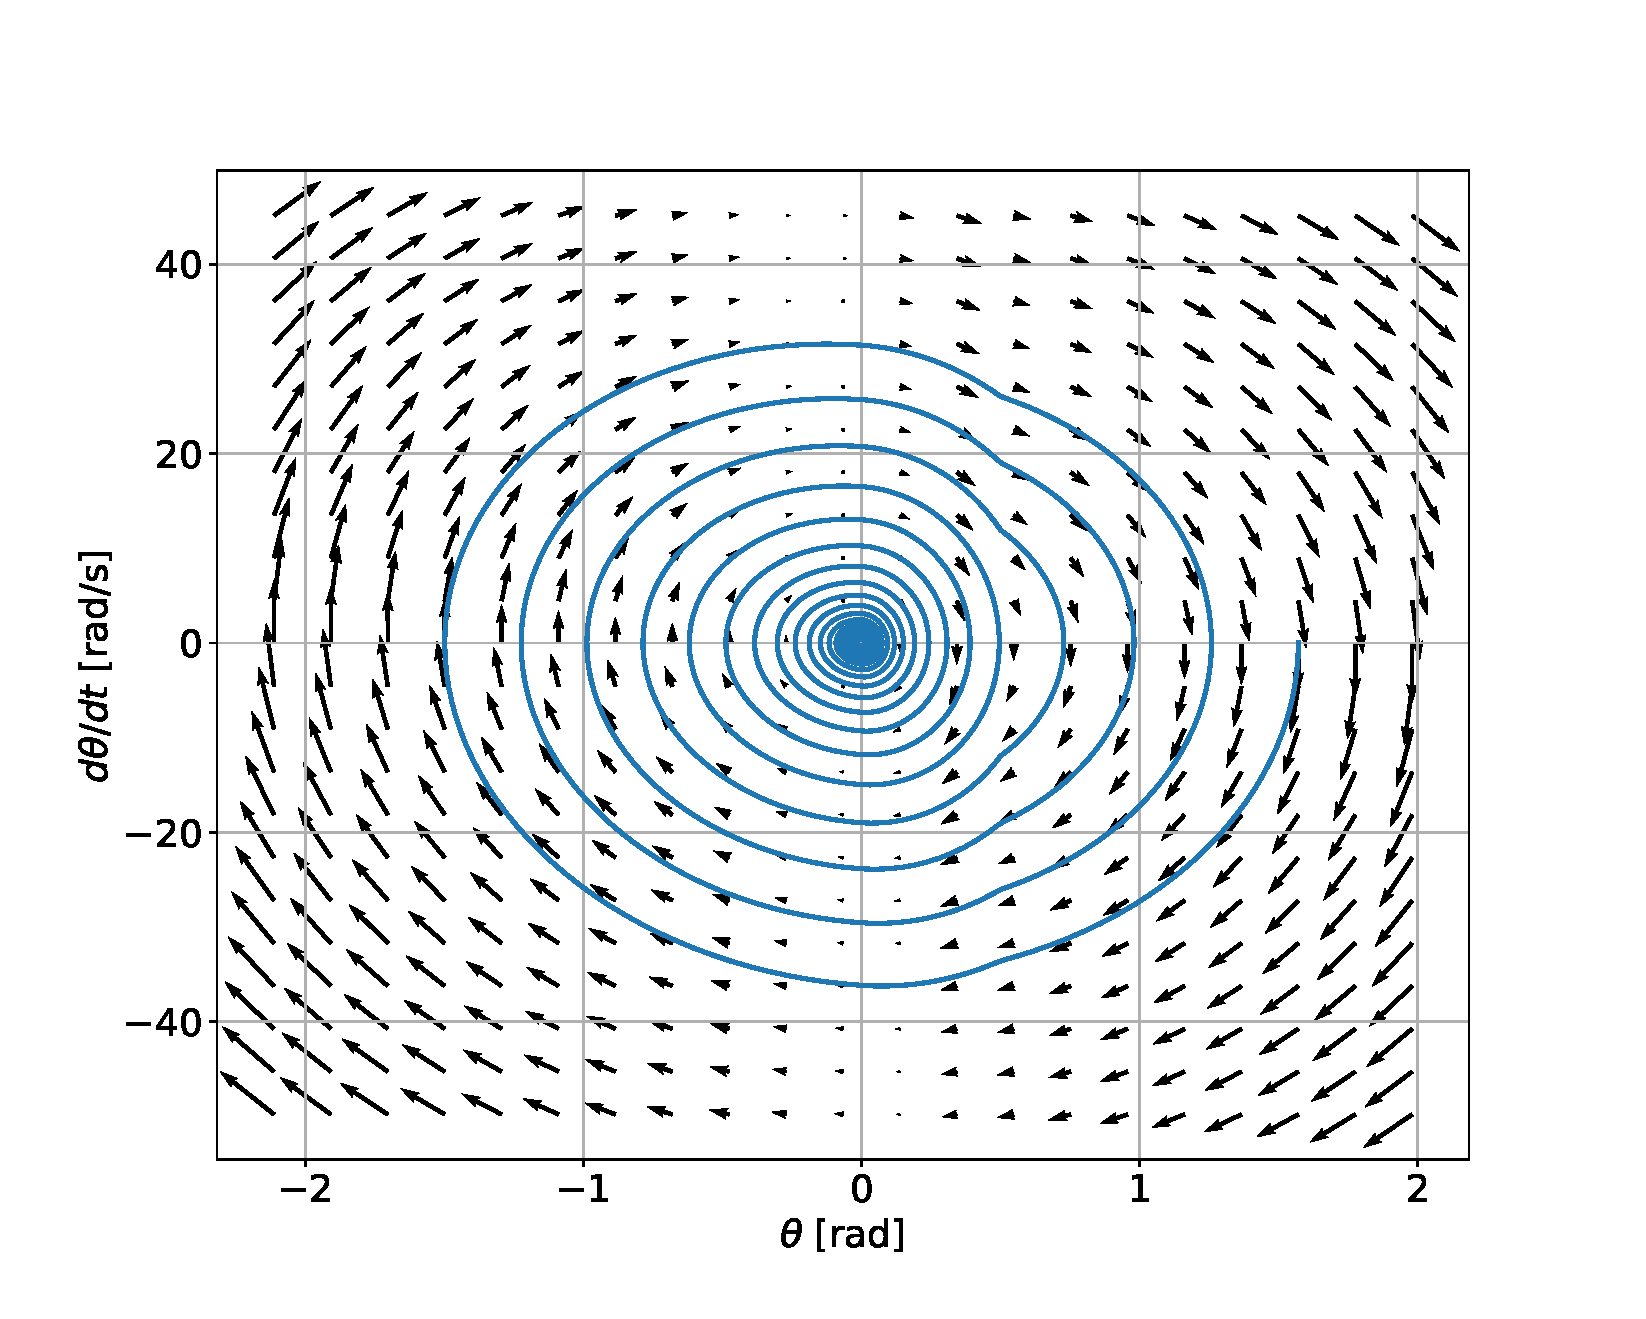
\includegraphics[height=2.8in]{1d_2.eps}
    \end{subfigure}
    \caption{Angle (state 0) and angular velocity (state 1) as a function of time, with associated phase portrait. System of pendulum with 2 springs and 2 dampeners. Initial conditions and parameters written on top of the left figure. Only one of the two dampeners (B2) is active.}
    \label{figure:1d}
\end{figure}

With dampeners in the system, the system loses angular velocity at each beat and tends to reach $\theta=0$, since gravity eventually takes over, in order to minimise the potential energy in the system. Figure \ref{figure:1d} shows a system with only one dampened spring, with $\theta_{ref} = 0.5$ rad. On the state plot, one can observe that the dampened system goes towards $\theta=0$ at equilibrium, which is the minimum of potential energy. On the phase portrait on the right, we observe that after starting with an initial position of $\pi/2$, there is a notch at $\theta=0.5$  rad. This is due to the system design: above its $\theta_{ref}$, a spring doesn't act on the system as it can only "pull" the pendulum. So above $\theta=0.5$ rad, the dampened spring with $\theta_{ref} = 0.5$ rad has no contribution, and when we reach this angle, the notch indicates that the dampening coming from this spring starts.

\begin{figure}[H]
	\centering
	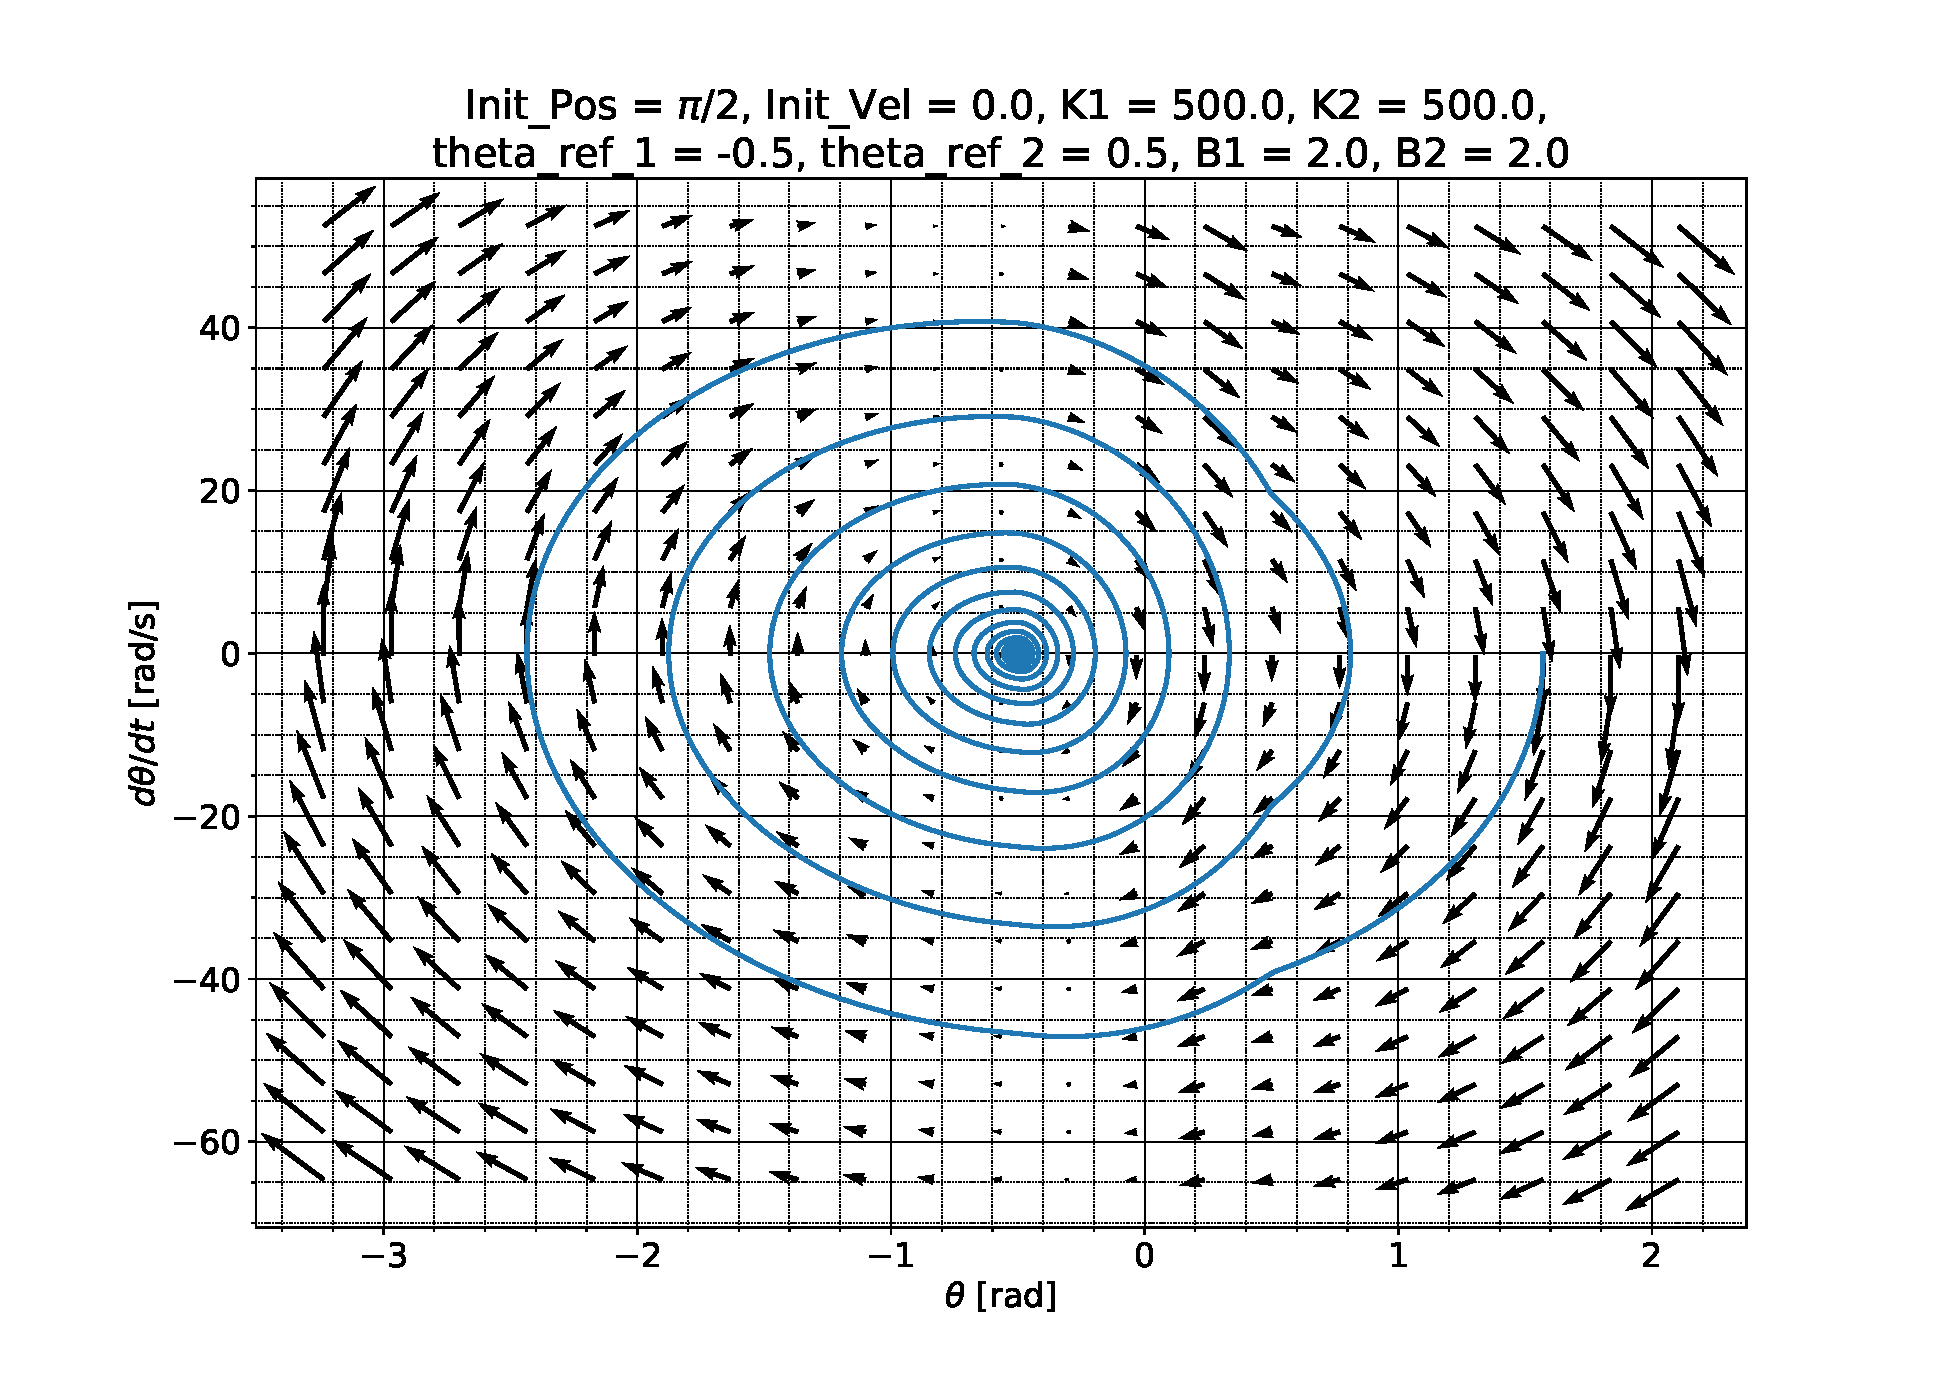
\includegraphics[width=0.6\linewidth]{1d_3.eps}
    \caption{Phase portrait of pendulum with 2 springs and 2 dampeners. Initial conditions and parameters written on top. The two dampeners (B1, B2) are active.}
	\label{figure:1d3}
\end{figure}

The Figure \ref{figure:1d3} shows the phase portrait of a double-damped system. As explained for figure \ref{figure:1d}, the system design implies that above $\theta = -0.5$ rad, the spring S2 has no contribution and that the same is true for the spring S1 below $\theta = 0.5$ rad. Hence, two notches are observable at $\theta_{ref1} = 0.5$ rad and $\theta_{ref2} = -0.5$ rad, and in-between those angles lies an interval within which there is no dampening occurring.

\subsection*{1.e Can you find a combination of spring constant ($K$),
  damping constant ($B$) and spring reference angle ($\theta_{ref}$) that
  makes the pendulum rest in a stable equilibrium at
  ($\theta = \pi/6$) radians? Describe the parameters used and support
  your response with relevant plots.}

\begin{figure}[H]
    \centering
    \begin{subfigure}[b]{0.5\textwidth}
        \centering
        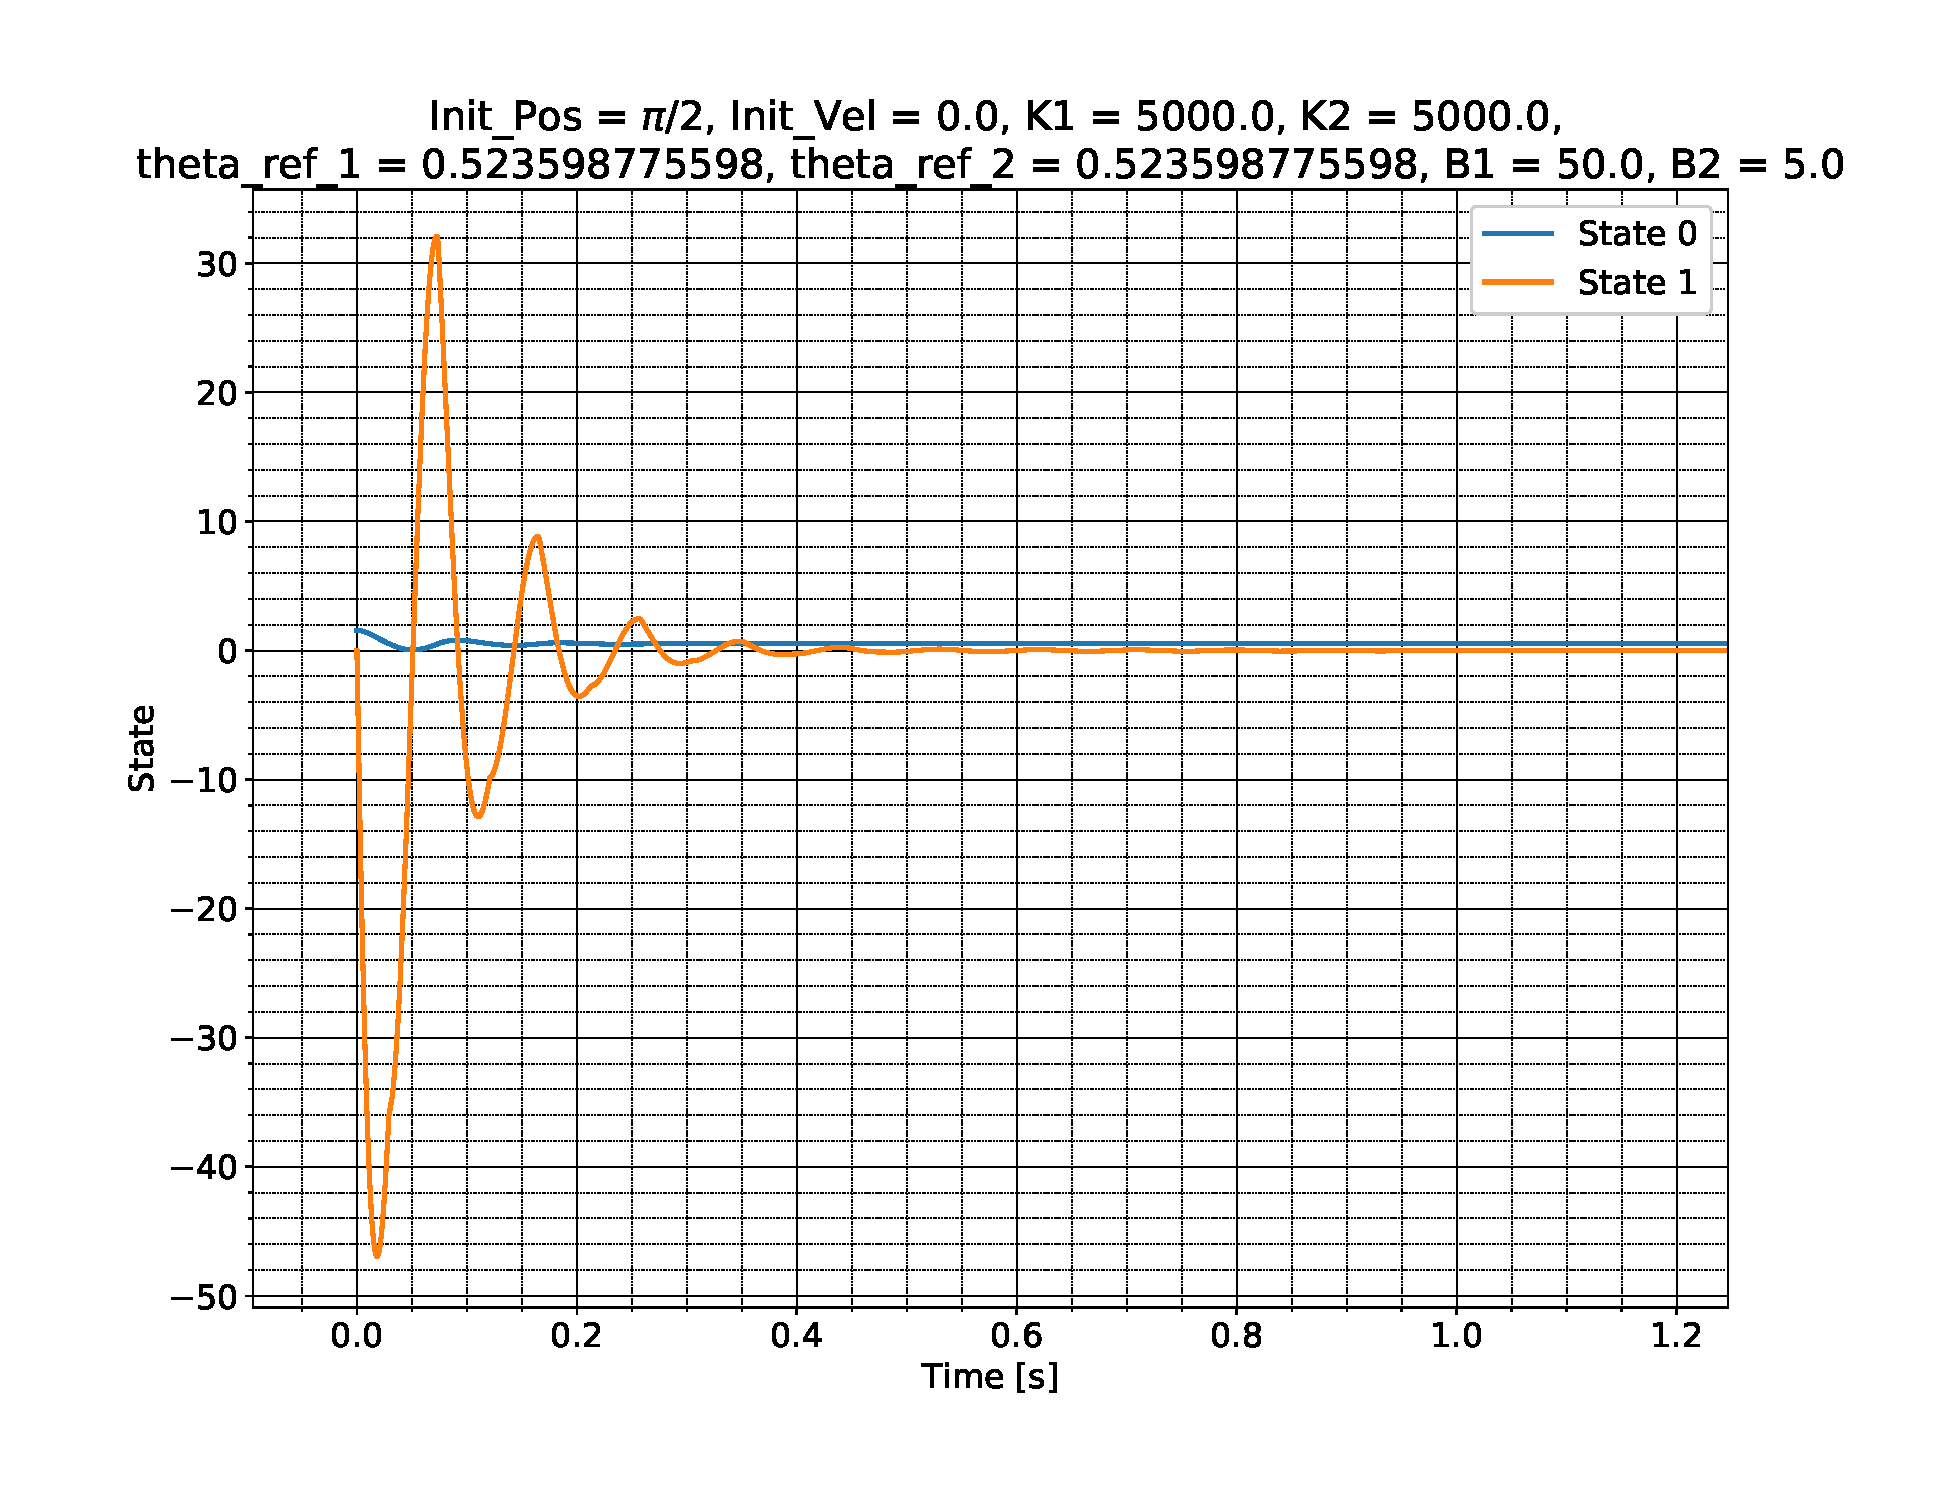
\includegraphics[height=2.8in]{1e_1.eps}
    \end{subfigure}%
    ~
    \begin{subfigure}[b]{0.5\textwidth}
        \centering
        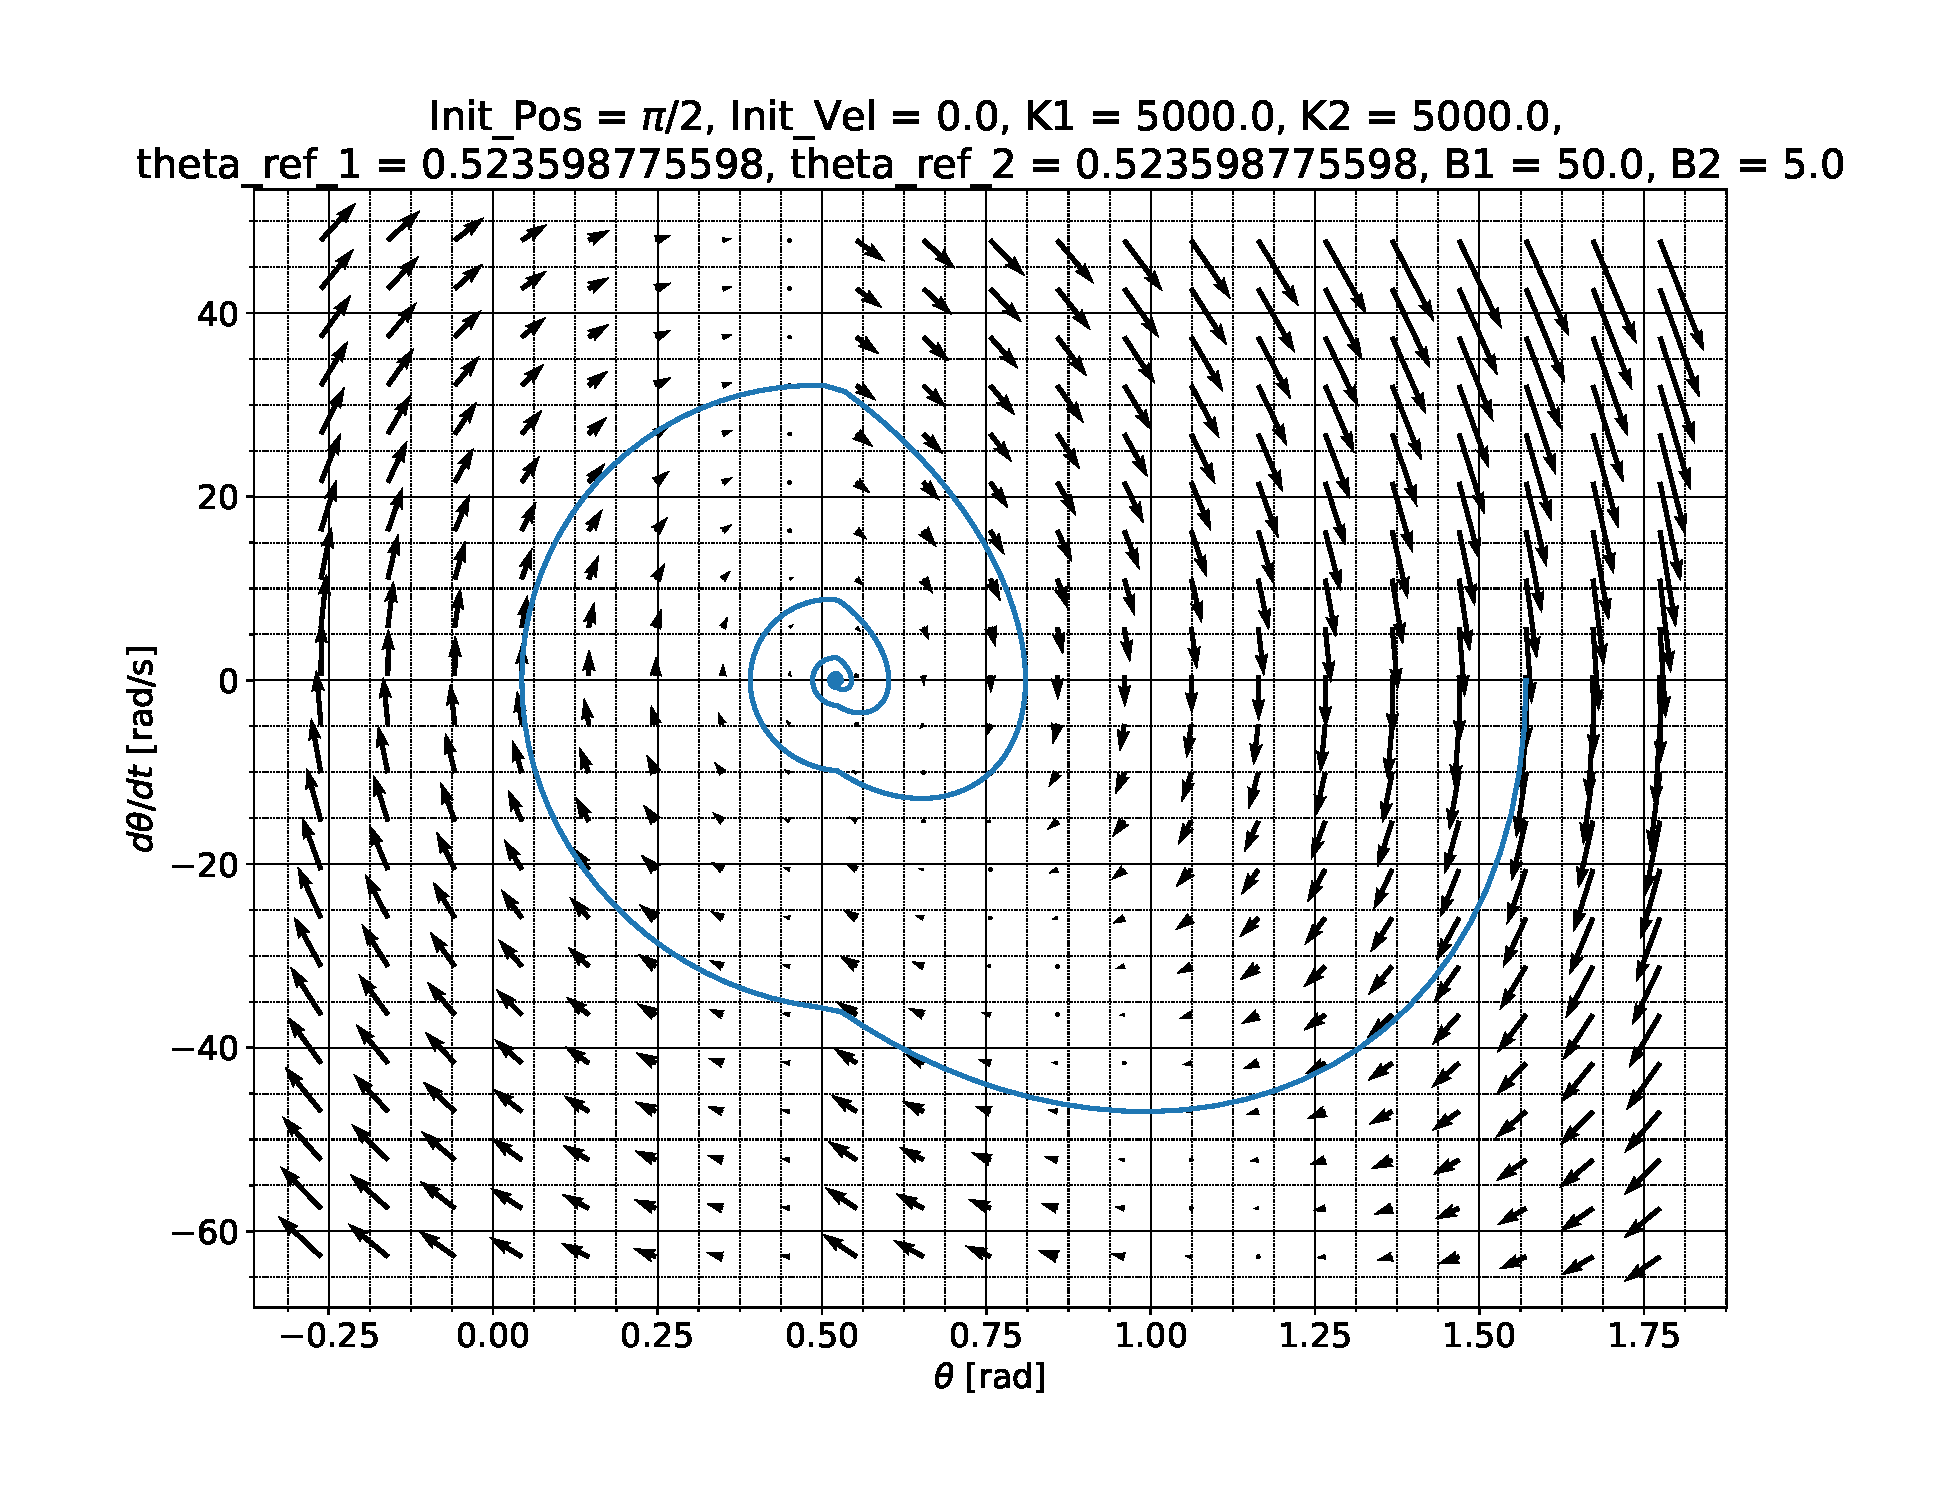
\includegraphics[height=2.8in]{1e_2.eps}
    \end{subfigure}
    \caption{Angle (state 0) and angular velocity (state 1) as a function of time, with associated phase portrait. System of pendulum with 2 springs and 2 dampeners. Initial conditions and parameters written on top of the left figure. Only one of the two dampeners (B2) is active.}
    \label{figure:1e}
\end{figure}

The system reaches a stable equilibrium at $\theta = \pi/6$, as seen in Figure \ref{figure:1e} for the following parameters:

\begin{equation}
\begin{split}
\theta_{ref1,2} = \pi/6 \hspace{2.5mm} & \hspace{2.5mm} K_{1,2} = 5000\\
B_{1} = 50 \hspace{2.5mm} & \hspace{2.5mm} B_{2} = 5
\end{split}
\end{equation}

Please note that other parameters variation (e.g. spring constant) could allow such a behavior.

\subsection*{1.f What is the missing component between a real muscle
  and the muscle model with passive components that you just
  explored? What behavior's do you lack because of this missing component?}

A real muscle combines passive and active elements to generate a force and resist contraction/elongation. In our spring/dampener model, we only have the passive elements that can respond to external constrains, but we don't have any mean to generate an active force - in other words, we cannot simulate the response of the muscle to an intern stimulus, e.g. coming from motor neurons.

\newpage
\section*{Exercise 2 : Hill muscle model}
\label{sec:question-2}

In exercise 1, you explored the role of different passive components
and the effects of its parameters on the system. In this exercise, we
try to understand the contractile or the active element of the hill
muscle model. The components of the hill muscle are described in
figure \ref{fig:hill_muscle}. The equations used to model the hill
muscle can be found in the pdf \fileref{HillMuscleEquations.pdf}


Use \fileref{exercise2.py}, \fileref{lab4\_mass.py},
\fileref{SystemParameters.py} and \fileref{Muscle.py} files to
complete the exercise.

\begin{figure}[H]
  \centering 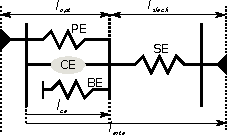
\includegraphics[scale=2.5]{figures/hill_muscle}
  \caption{Hill muscle model}
  \label{fig:hill_muscle}
\end{figure}

Where,

\begin{itemize}
\item $PE$ : Parallel element (Prevents muscle from over stretching)
\item $BE$ : Muscle Belly (Prevents muscle from collapsing on itself)
\item $SE$ : Series element or the muscle tendon element
\item $CE$ : Contractile Element or the active element
\item $l_{opt}$ : Muscle optimal fiber length
\item $l_{slack}$ : Muscle tendon slack length
\item $l_{CE}$ : Contractile element length
\item $l_{MTC}$ : Muscle Tendon Complex length
\end{itemize}


\begin{figure}[H]
  \centering
  \begin{subfigure}[b]{0.49\textwidth}
    { \centering
      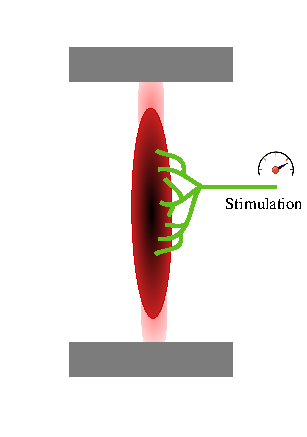
\includegraphics[width=\textwidth]{figures/isometric_muscle}
      \label{fig:isometric_muscle}
    }
    \caption{Isometric muscle setup :\\ To study the relationship
      between Force-Length.}
  \end{subfigure}
  \begin{subfigure}[b]{0.49\textwidth}
    { \centering
      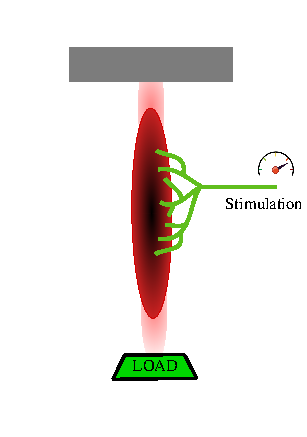
\includegraphics[width=\textwidth]{figures/isotonic_muscle}
      \label{fig:isotonic_muscle}
    }
    \caption{Isotonic muscle setup :\\ To study the relationship
      between Force-Velocity.}
  \end{subfigure}
  \caption{Muscle Length-Velocity-Force Setup}
  \label{fig:muscle-setup}
\end{figure}

\subsection*{Muscle Force-Length Relationship}
\label{sec:muscle-force-length}
In this exercise you will explore the relation between the length and
velocity of the muscle. In order to do this we replicate the set-up
show in figure \ref{fig:muscle-setup}. Here the length of the muscle is
held constant by attaching it's tendon to two fixed points. While
applying a constant stimulation, observing the force produced will
give the relationship between muscle contractile element length and
force.
\subsection*{2.a For a given stimulation, explore the relationship
  between active and passive muscle forces and the length of the
  contractile element.  Plot the force-length relationship curve.
  Discuss the different regions in the plot}

\begin{figure}[H]
\centering
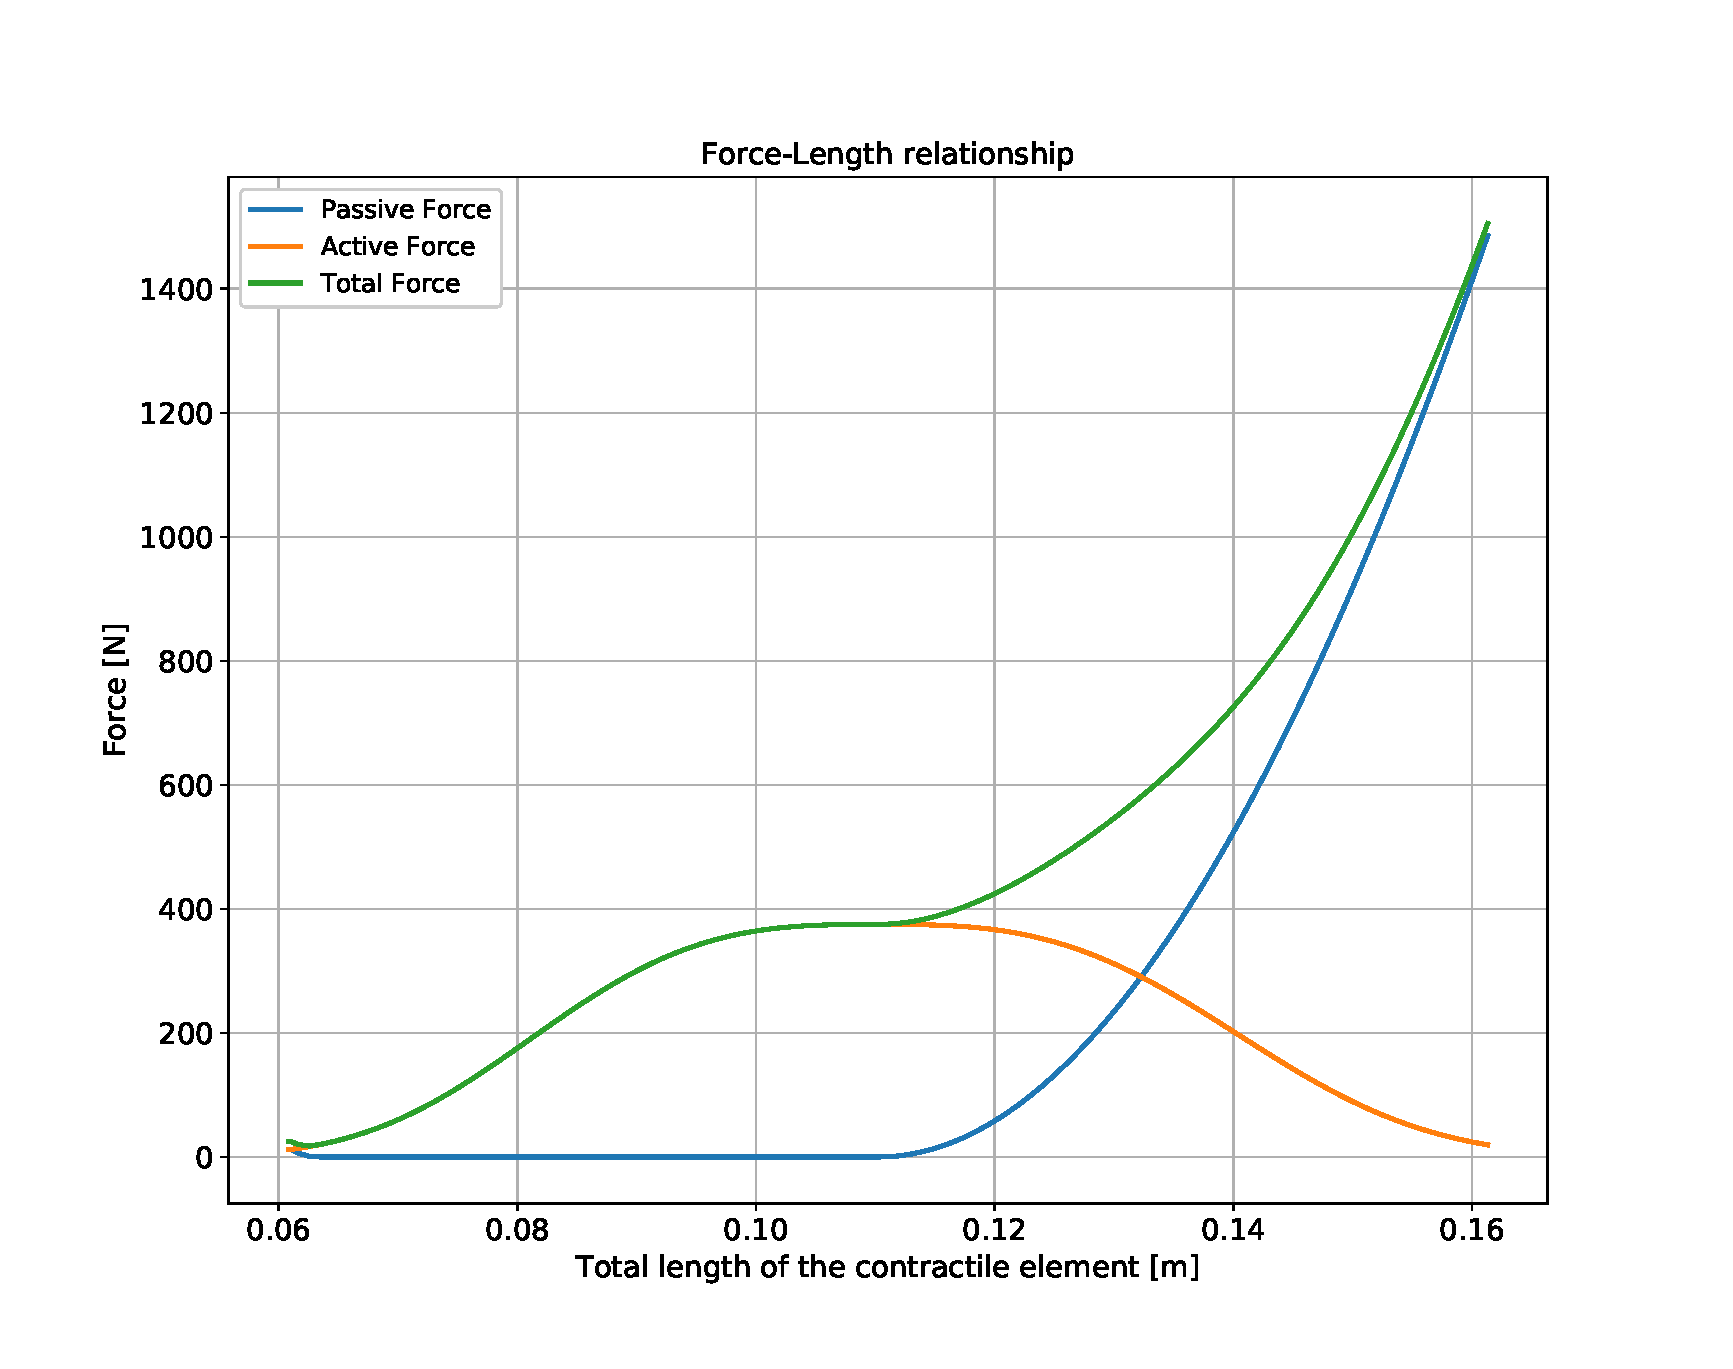
\includegraphics[width=0.8\linewidth]{2a.eps}
\caption{Various forces (passive, active, total) as a function of total length of the contractile element, in an isometric montage. Parameters used here are $l_{opt} = 0.11$ m and activation $=0.25$. Total length of the contractile element goes from $95\%$ to $105\%$ of original length $l_{CE}$.}
\label{figure:2a}
\end{figure}

As seen in figure \ref{figure:2a}, the active force increases until reaching a plateau near 400 N, at approx 10 cm. Then, it starts to decrease shortly before 12 cm. At the same length, the passive force starts to increase rapidly, having a bigger contribution to the total force than the active force has. The middle point of the plateau -- 11 cm -- corresponds to the optimal size of the contractile element. The active force has a bell shape because of the muscle's histology: when too short, actin filaments overlap and hit the Z-disc of the sarcomere, incapacitating the myosin heads to further pull the actin and shorten the sarcomere, already compressed at maximum; when the contractile element is too extended,  myosin heads simply loose contact with the actin filaments, and the muscle is then incapable  of generating an active force. In-between those two extreme cases, lies the case where the myosin/actin contact is optimized and the muscle can generate a maximum active force -- the extension corresponds to $l_{opt}$, the optimal muscle fiber length. After a certain point of extension, the muscle will start to oppose a passive force to counteract its elongation. In result and since the Hill's muscle model equation for the passive force goes with the square of the contractile element's length $l_{ce}$, the passive force evolves more rapidly than the active force.
 
\pagebreak
\subsection*{2.b In (2.a), you explored the muscle force-length
  relationship for a given stimulation. What happens to the
  relationship when the stimulation is varied between [0 - 1]? Supportt
  your response with relevant plots.}

\begin{figure}[H]
\centering
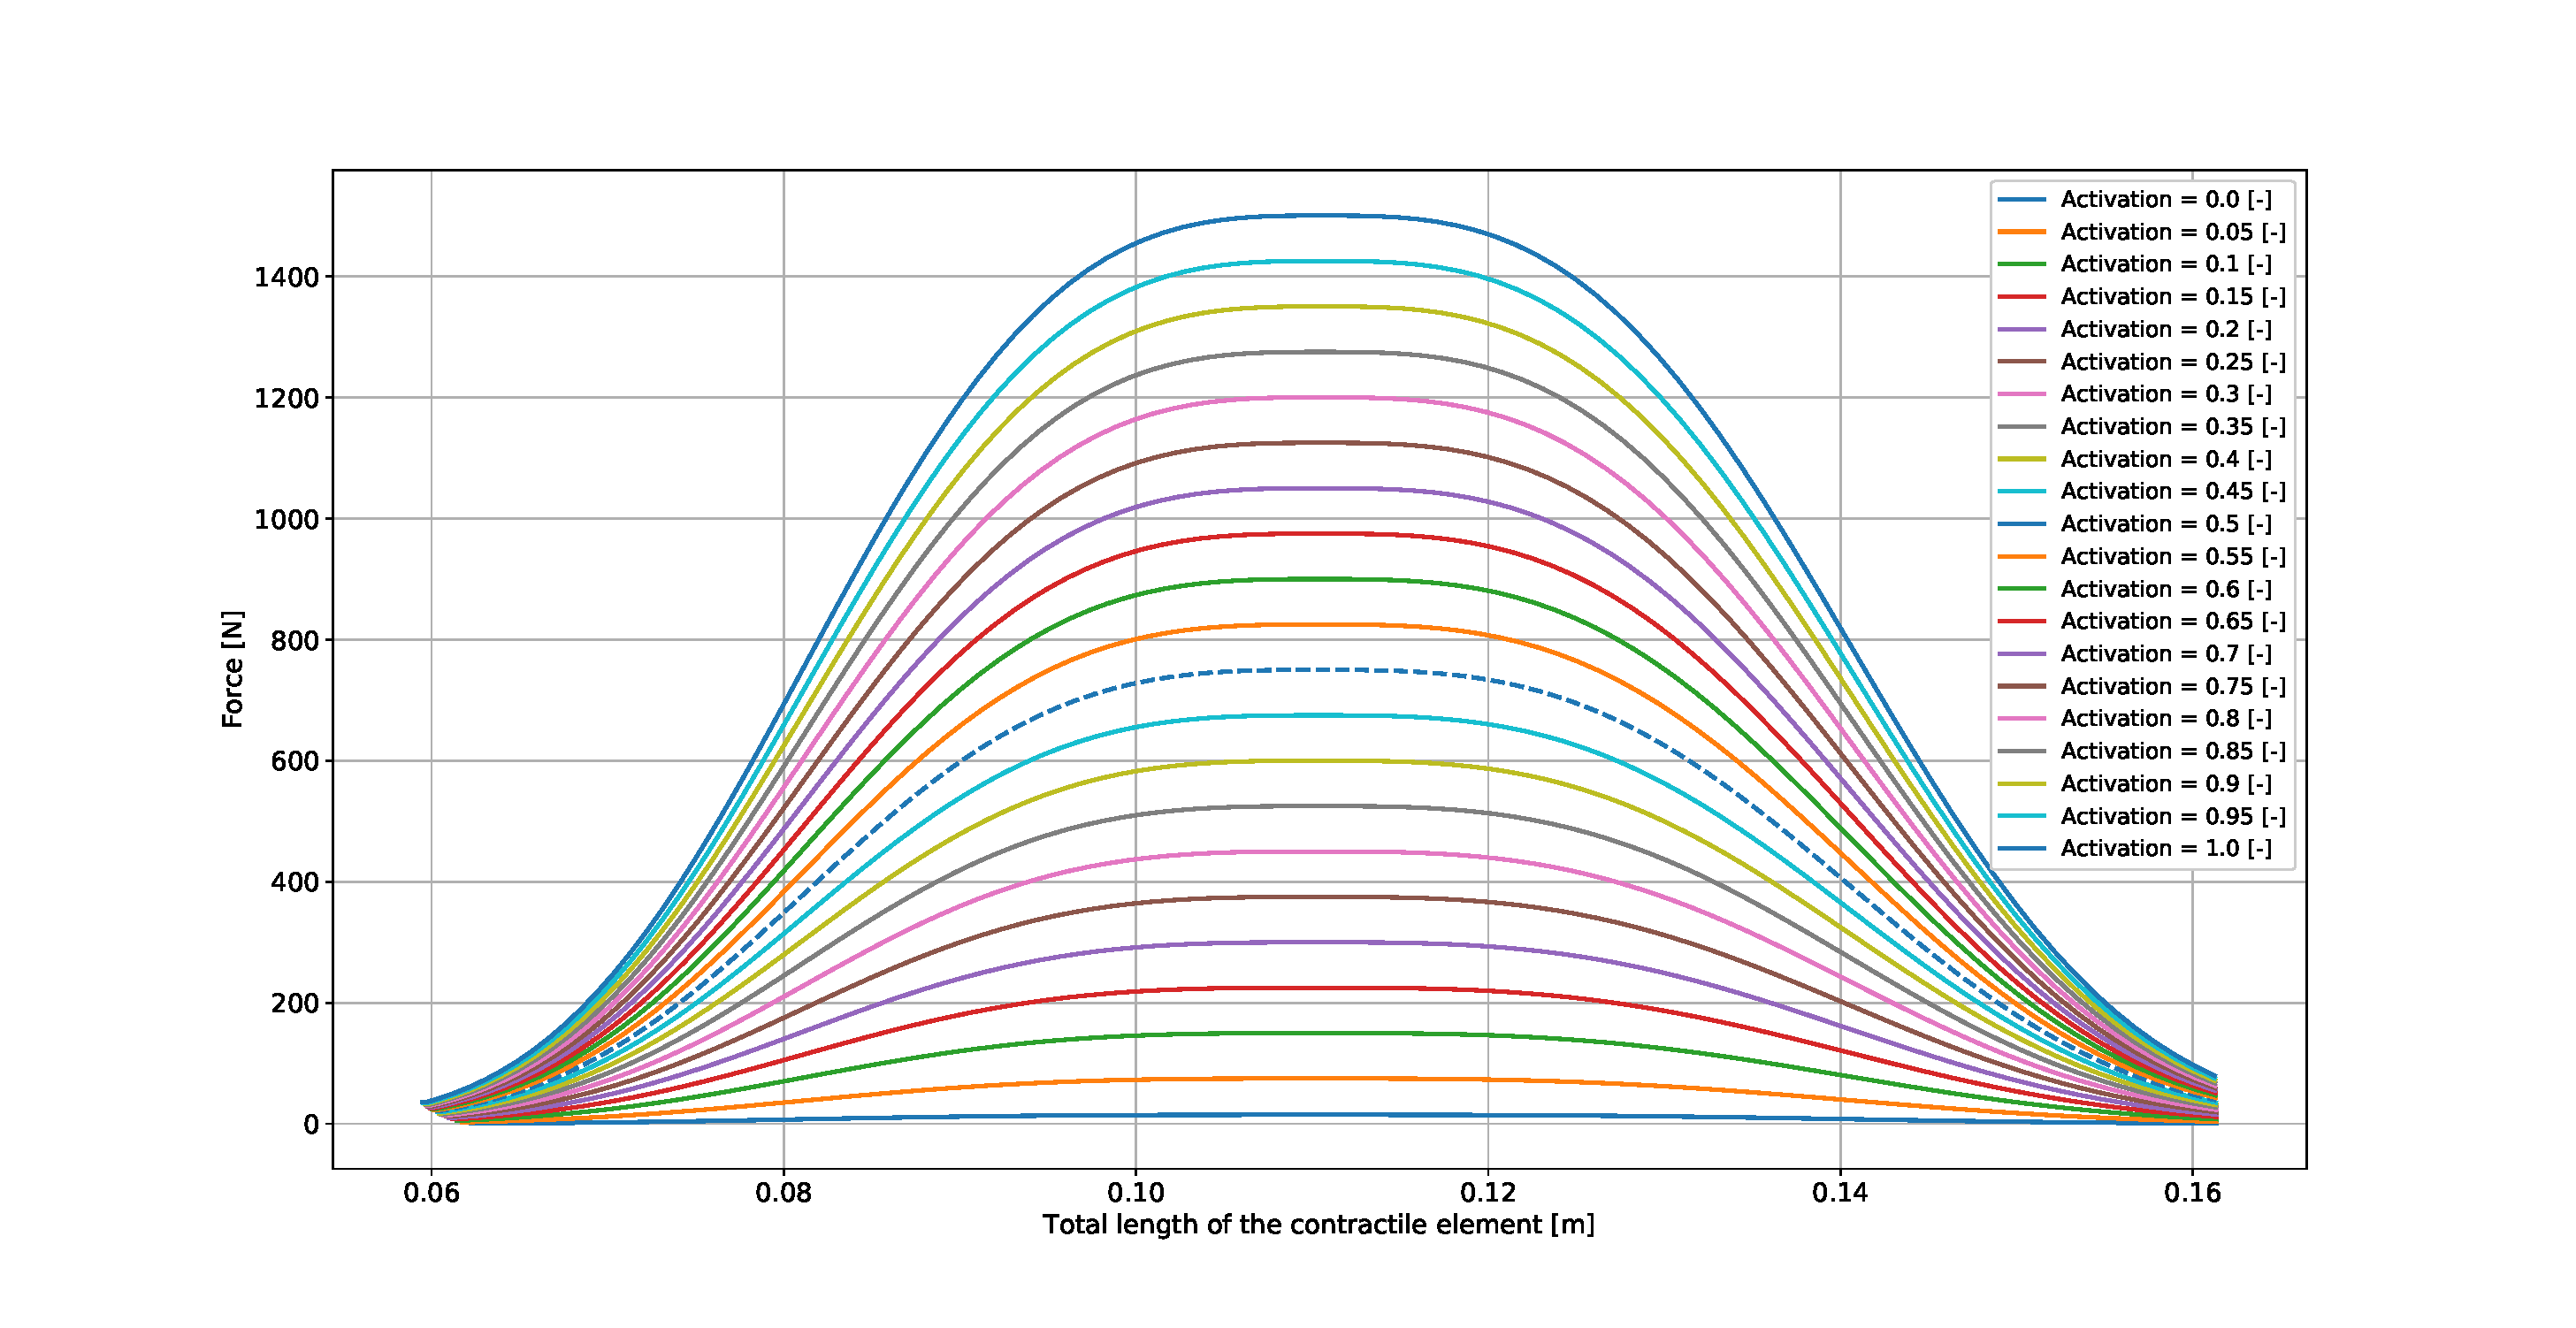
\includegraphics[width=\textwidth]{2b.eps}
\caption{Evolution of the active force for activation values (input stimulation) ranging from 0 to 1. The middle activation ($a = 0.5$) is represented with a dashed line for visual purposes. Activation represents a normalized spiking rate originating from motor neurons connected to the muscle.}
\label{figure:2b}
\end{figure}

In Figure \ref{figure:2b}, one can see that with increasing activation, the active force exhibits a higher, but also a wider bell shape. The maximum of the active force, reached when the activation equals 100\%, is 1500 N, which is the maximal force that the muscle can generate -  it is a parameter of the muscle than can be tempered with if necessary.

The activation parameter affects only the active force generated by the muscle's contractile element ($F_{ce}$), as governed by the following equation:

\begin{equation}
F_{ce} = A \cdot F_{max} \cdot f_l(l_{ce}) \cdot f_v(v_{ce})
\end{equation}

The difference between the maximum active force and the maximum passive force for a stretch range of 95\% to 105\% of the contractile element's length decreases with increasing activation values, as shown in Figure \ref{figure:2b2}, confirming that the passive force isn't influenced by this parameter while the active force is directly depending on it. 

\begin{figure}[H]
\centering
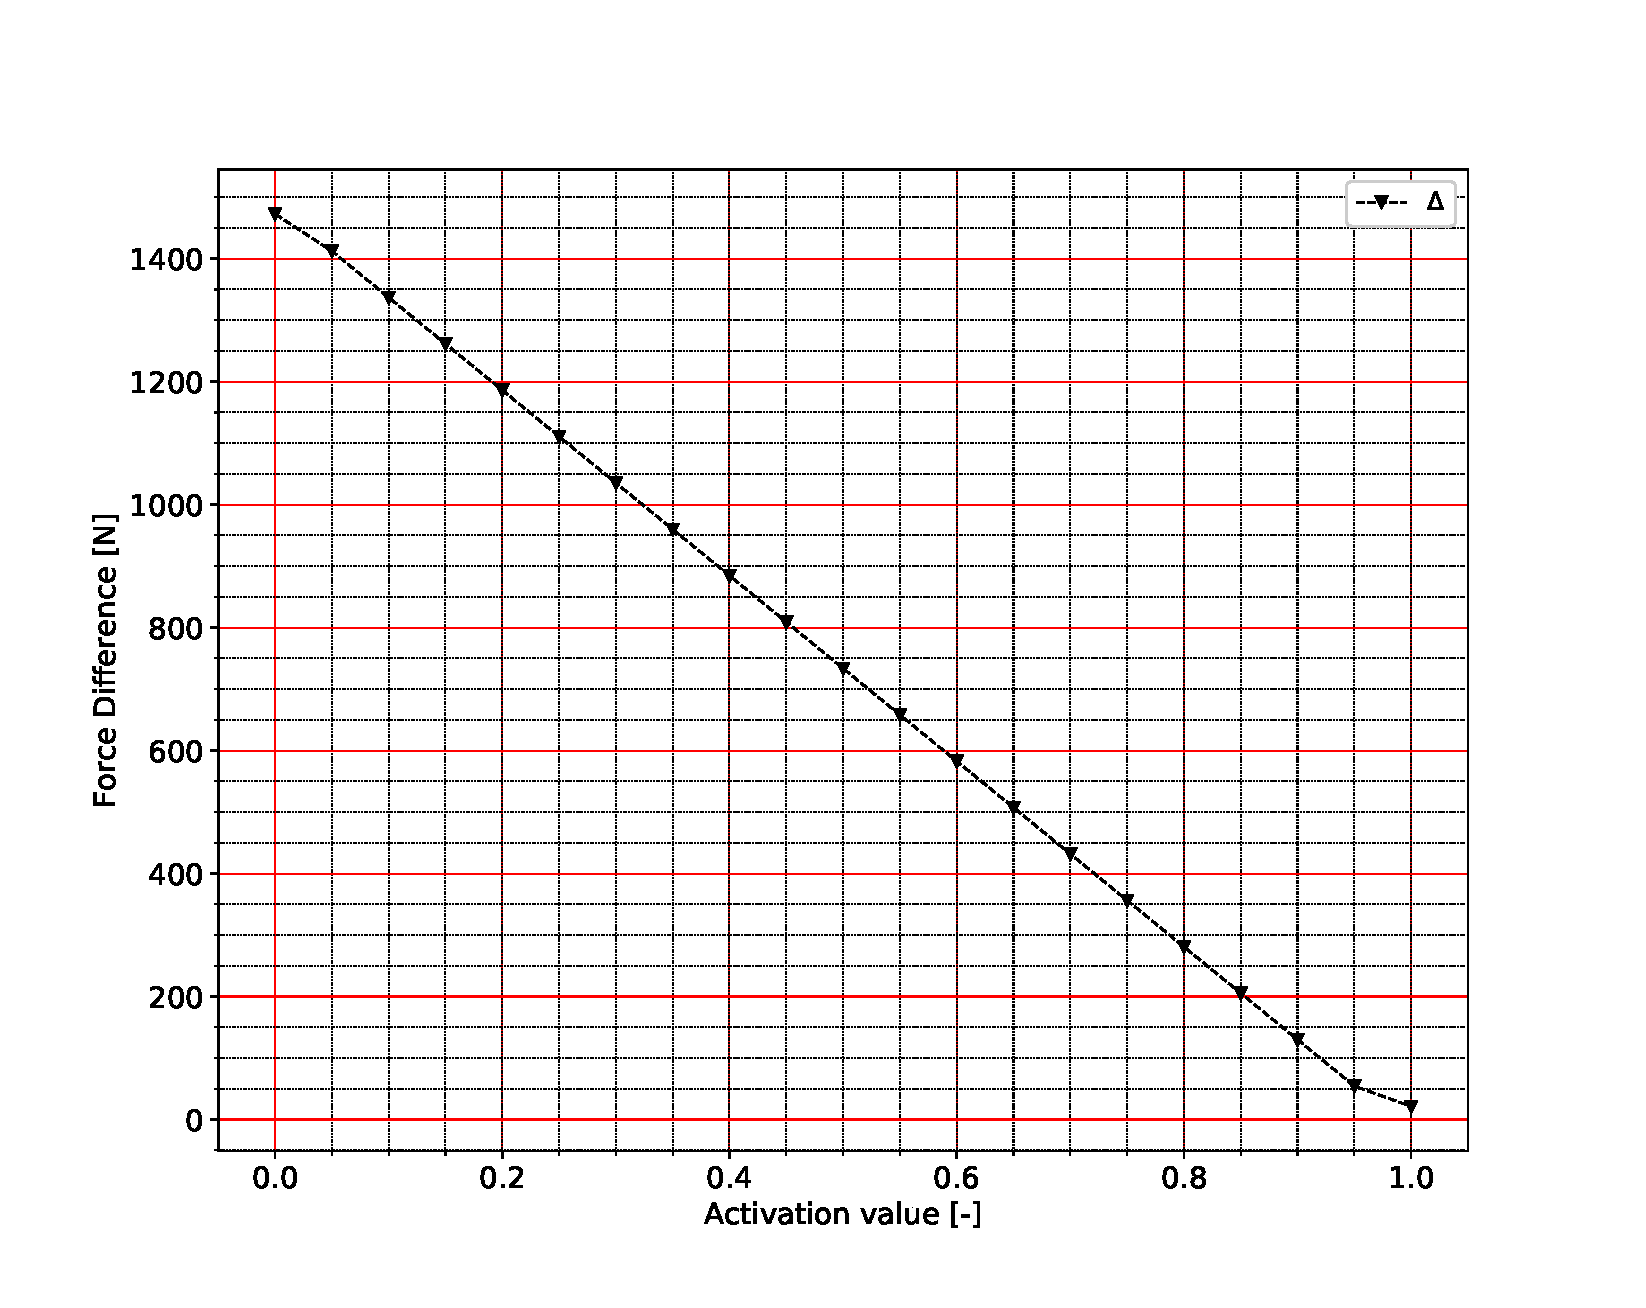
\includegraphics[width=0.6\textwidth]{2b_2.eps}
\caption{Difference between the maximum value of the active force and the passive force as a function of the activation value.}
\label{figure:2b2}
\end{figure}

\subsection*{2.c Describe how the fiber length ($l_{opt}$) influences
  the force-length curve.  (Compare a muscle comprised of short muscle
  fibers to a muscle comprised on long muscle fibers.)}

\begin{figure}[H]
\centering
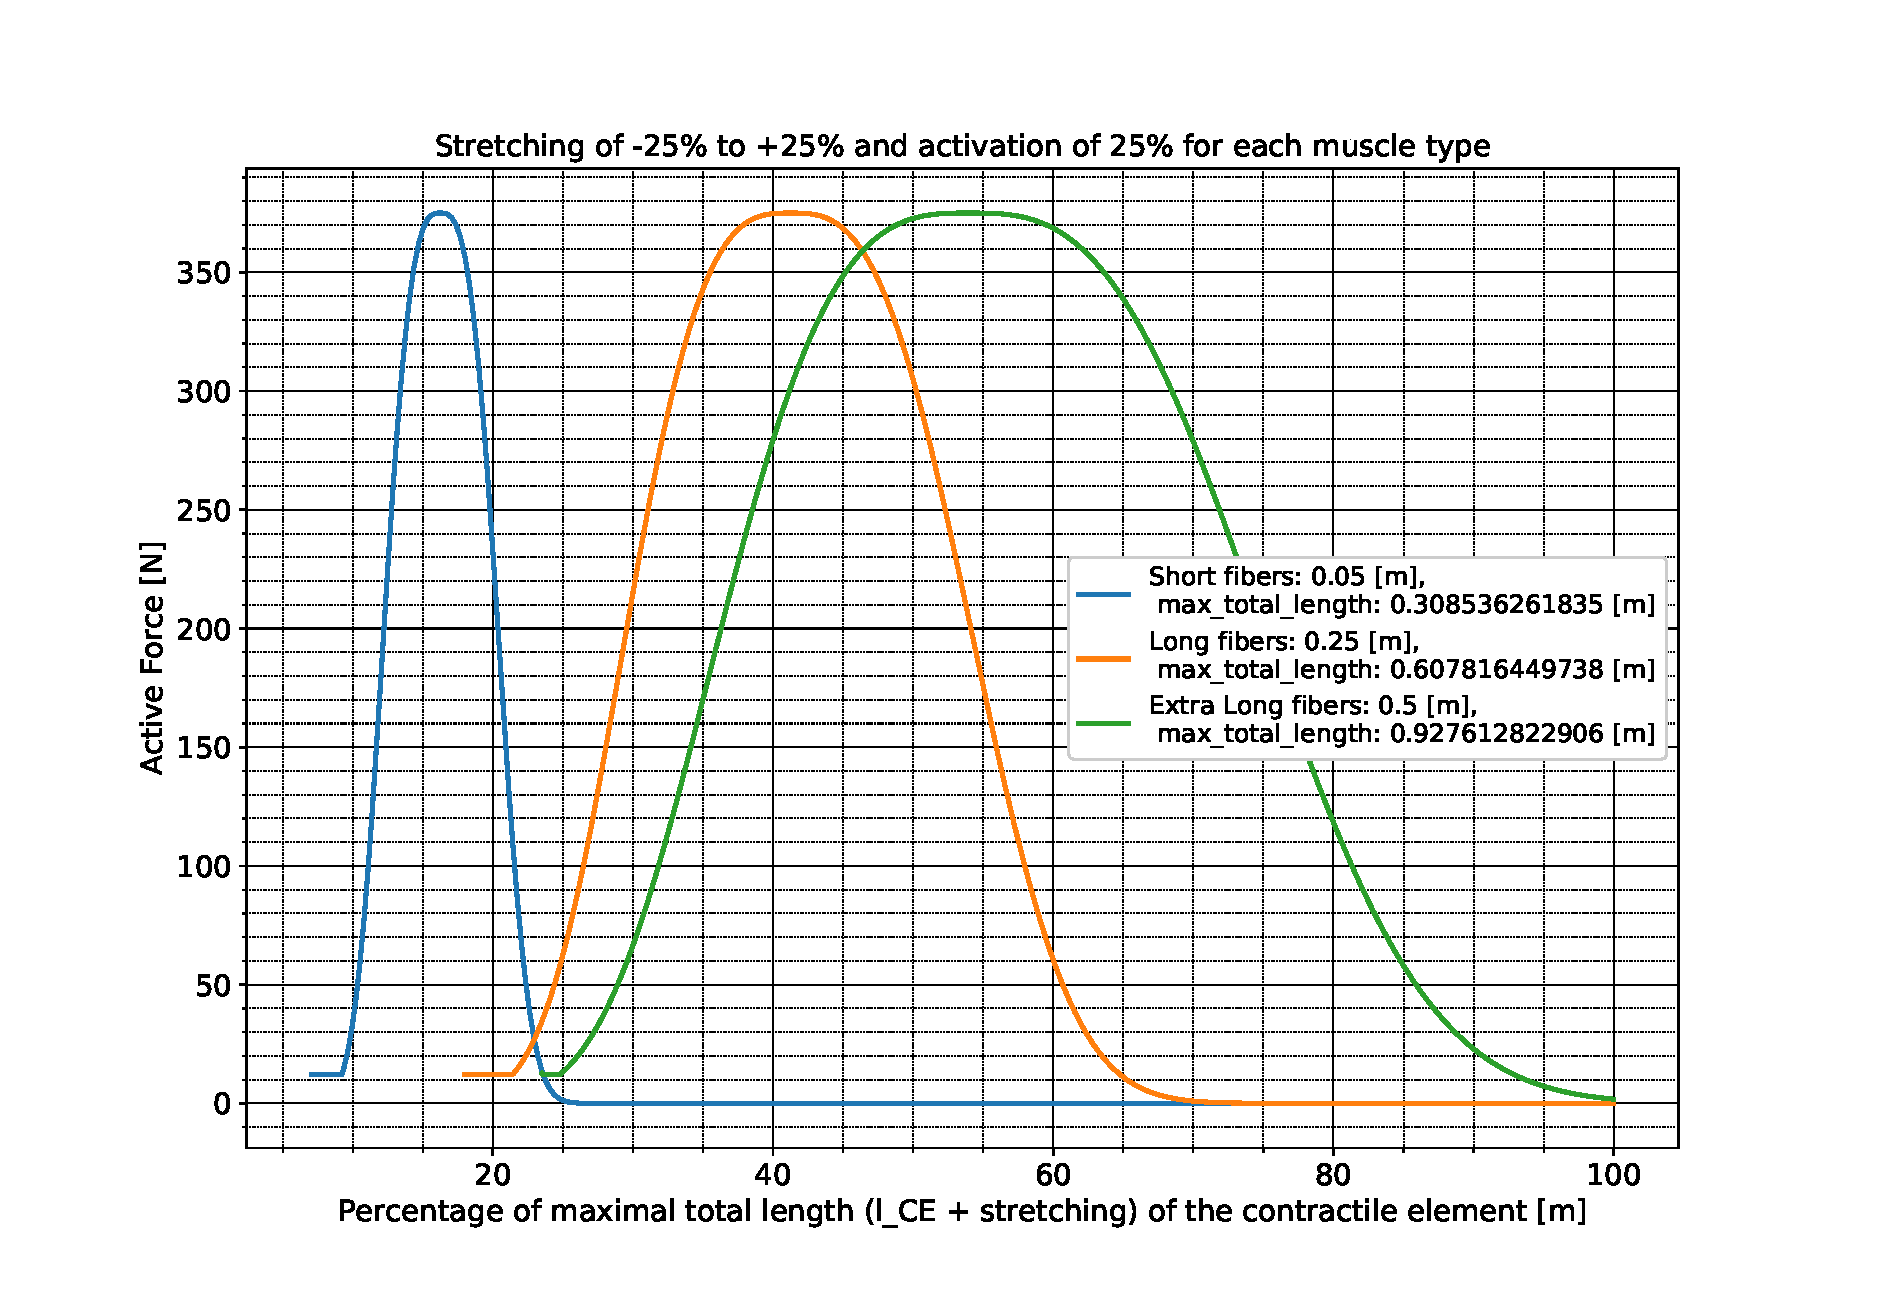
\includegraphics[width=0.8\textwidth]{2c_1.eps}
\caption{Stretching of 75\% to 125\% of the contractile element's original length, with an activation of $a=0.25$, for three muscle types, constituted of short ($l_{opt}=0.05$m), long ($l_{opt}=0.25$m) or extra long ($l_{opt}=0.5$m) muscle fiber length. The plot shows the normalised elongation, in order to better compare them.}
\label{figure:2c1}
\end{figure}

\begin{figure}[H]
\centering
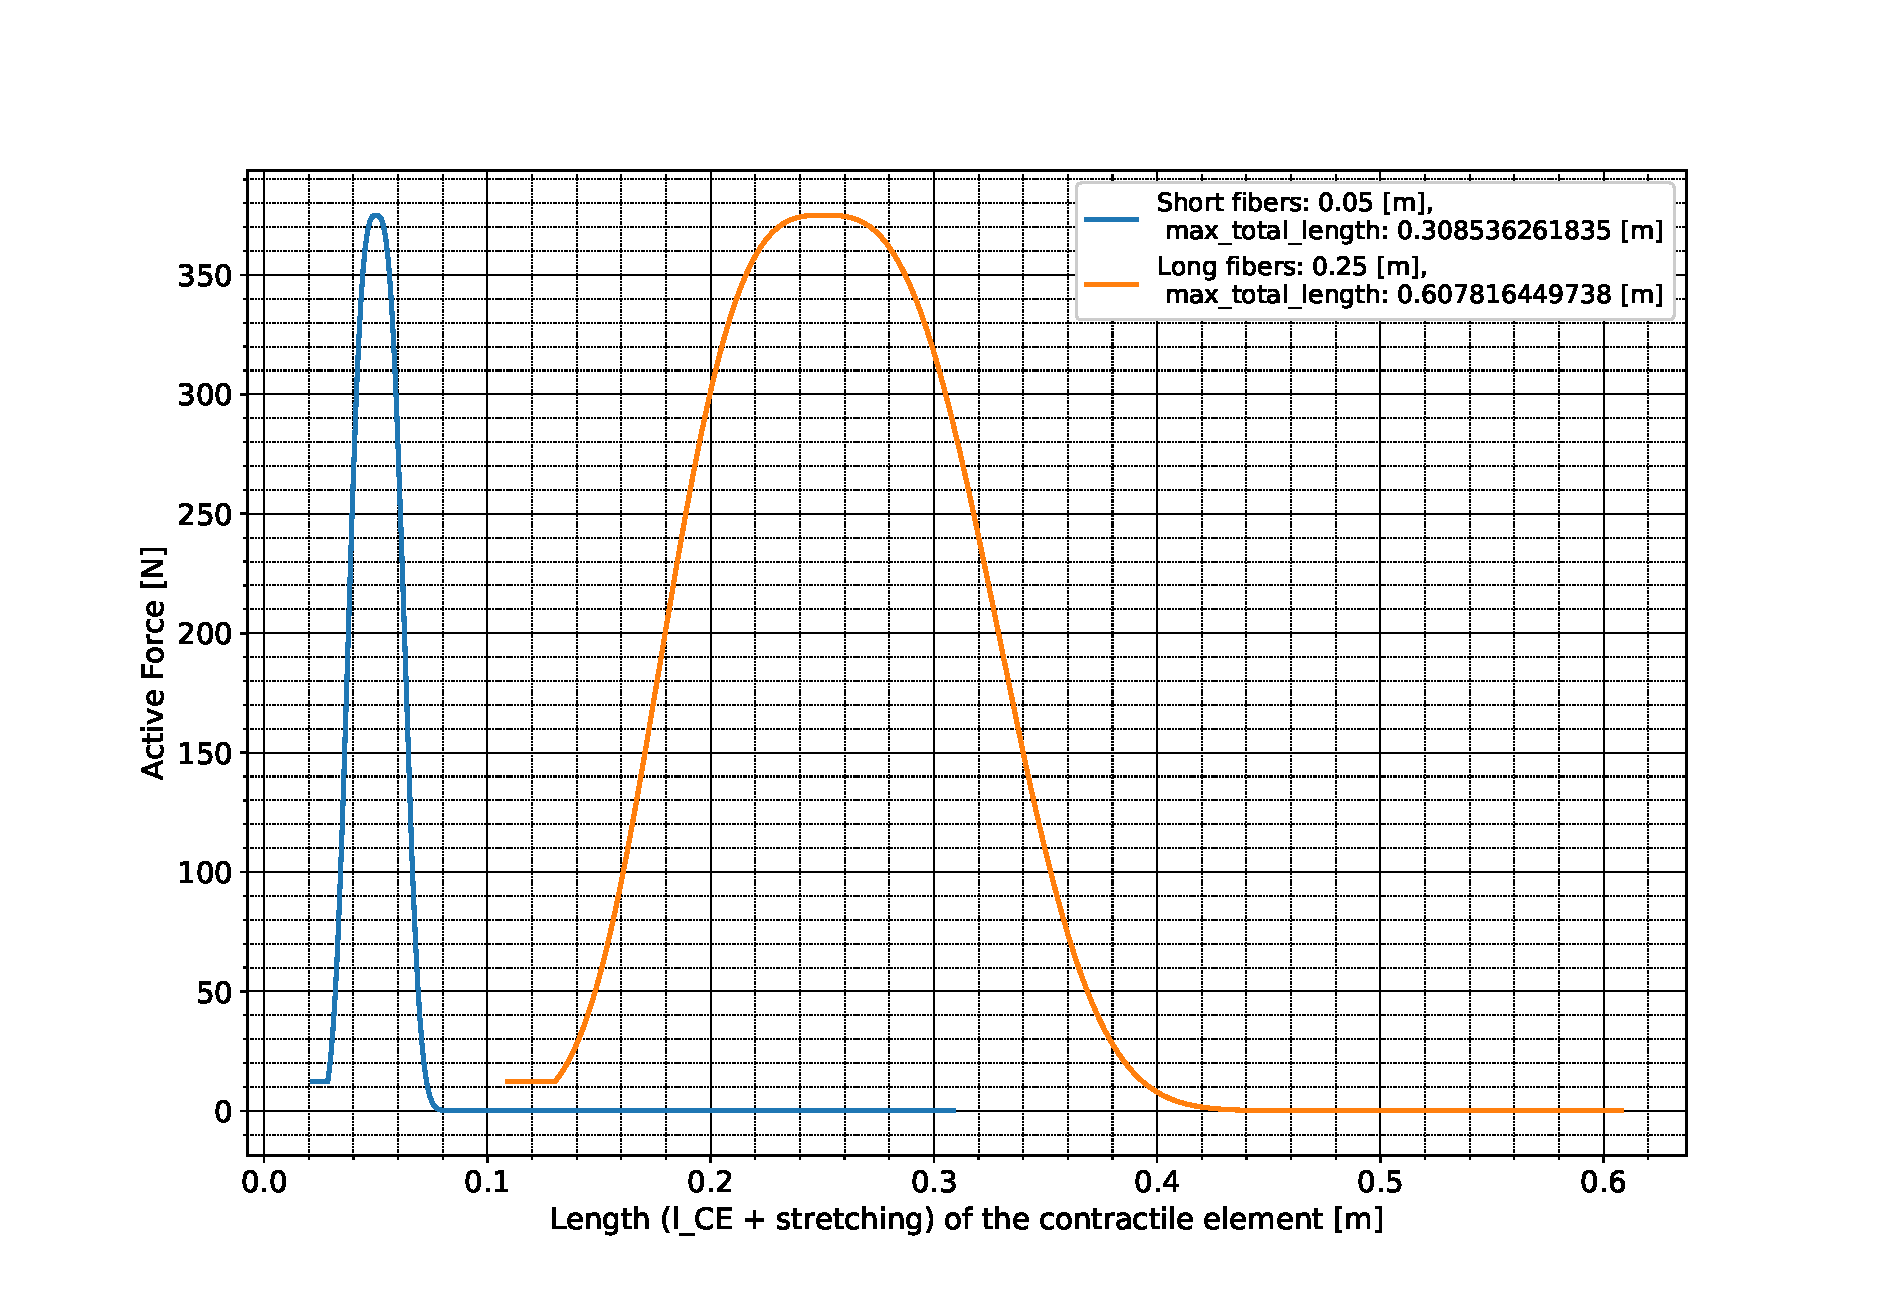
\includegraphics[width=0.8\textwidth]{2c_2.eps}
\caption{Stretching of 75\% to 125\% of the contractile element's original length, with an activation of $a=0.25$, for the short ($l_{opt}=0.05$m) and long ($l_{opt}=0.25$m) muscle fiber types. Here, the representation of the elongation is absolute, in order to see the value corresponding to the middle of the maximal force plateau for the two different muscles.}
\label{figure:2c2}
\end{figure}

In Figure \ref{figure:2c1}, the plot of active force over elongation for three types of muscle with varying optimal muscle fiber lengths is shown. As the elongation is normalised for all three muscles -- the total elongation, that depends on several factors other than the optimal muscle fiber length only, is indicated on the graph for each muscle type -- we can easily compare them: a muscle with short muscle fiber length ($l_{opt}=5$cm) will rapidly (after 25\% of its max elongation, which is 7.7 cm) be unable to generate a force due to lost contacts between the actin filaments and the myosin heads. As the muscle fibers are small, the active force dynamics shape a narrow bell. As we increase the muscle fiber length, we observe that the bell shape widens and that the slope to get to the maximal value gets less steep. Furthermore, we observe a plateau at the maximum active force value that gets wider with increasing fiber length. However, this maximum value does not change from short to long or even extra long muscle fiber length, hinting that the maximum force does not depend on the fibers length. An absolute representation of the impact of muscle fiber length on the force dynamic such as in Figure \ref{figure:2c2} allows to see that the middle of the maximum force plateau corresponds to the optimal muscle fiber length ($l_{opt}$), which are equal to 5 cm for the "short" muscle and 25 cm for the "long" muscle. If we go back to Figure \ref{figure:2b}, we can confirm that the middle of the plateau for the maximum active force corresponds to the optimal muscle length then (which was $l_{opt}=0.11$m).

One can hypothesize that longer muscle fibers allow a muscle to be more versatile, in that its milder dynamic slope allows a better tuning of the force, and that its bigger plateau grants the ability to sustain the maximum force for a wider range of muscle stretch. Conversely, short muscle fibers would imply a more all-or-nothing type of movement, since the dynamic range is narrower. Indeed, the limit case where the muscle fiber would be infinitely small implies that the muscle would generate the maximal force in an infinitely short range, resembling a Dirac impulse. 

\subsection*{Muscle Velocity-Tension Relationship}
In this exercise you will explore the relation between the force and
velocity of the muscle. In order to do this we replicate the set-up
show in figure \ref{fig:muscle-setup}. Here the length of the muscle is
allowed to vary by attaching one of its end to a fixed point and the
other to a variable external load. While applying a constant load
initially and holding the muscle at constant length, a quick release
is performed to let the muscle contract and pull the weight. The
maximum velocity during this quick release will give us the
relationship between muscle contractile velocity and the force

\subsection*{2.d For a stimulation of 1.0 and starting at optimal
  muscle length, explore the relationship between contractile element
  velocity and external load. Plot the Velocity-Tension relationship
  curve. Include shortening and lengthening regions}

\begin{figure}[H]
\centering
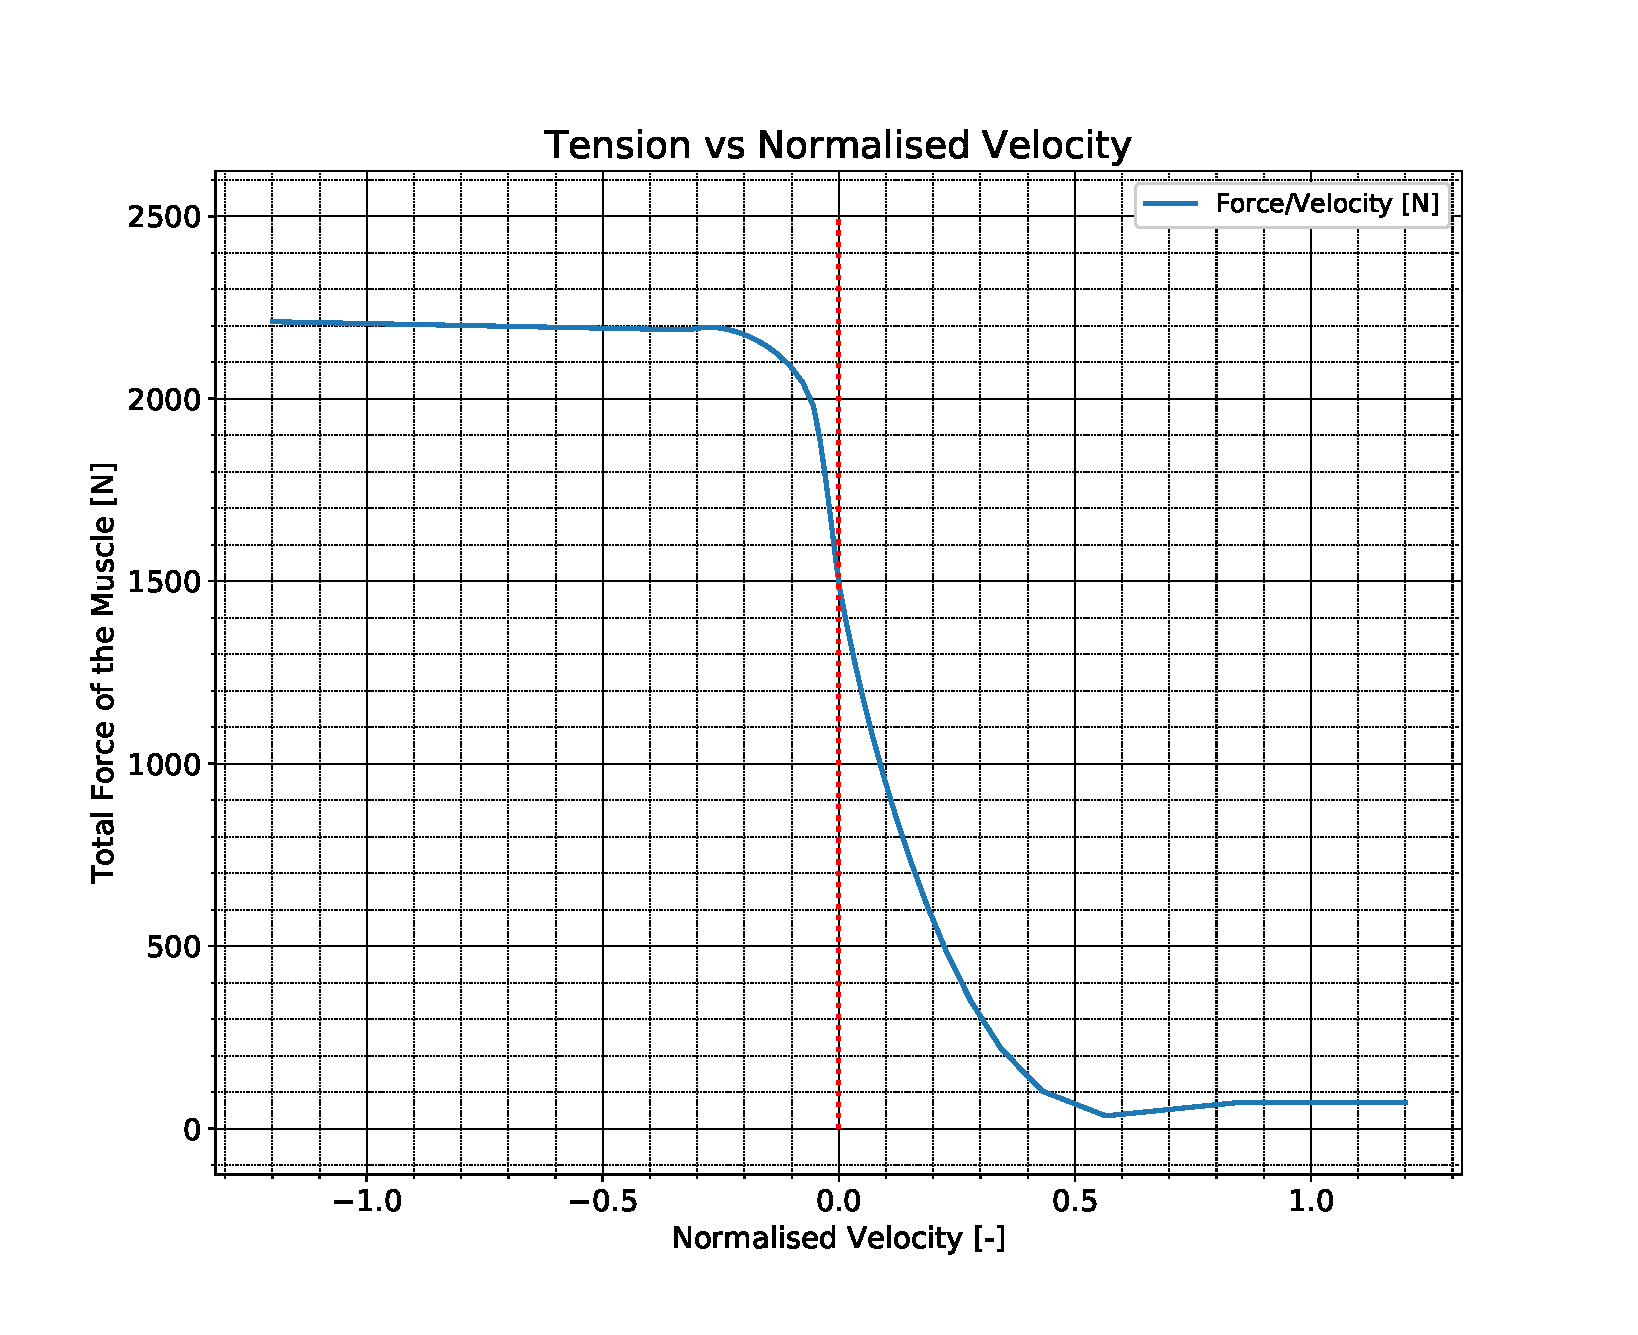
\includegraphics[width=0.8\textwidth]{2d_1.eps}
\caption{Plot of the relationship between the total force (active + passive) and the velocity. The velocity is related to the applied load and is normalised with respect to the maximum velocity achievable by the muscle ($v_{max}=1.2$ms\textsuperscript{-1}), and is directional: a minus sign implies a movement downwards, whereas a positive velocity is directed upwards (see Figure \ref{fig:muscle-setup}). A velocity of 0.0 corresponds to the isometric case. The external load applied to the muscle ranges from 1 to 321 kg, with steps of 10 kg. Muscle fiber length was fixed at $l_{opt} = 11$ cm and the activation at max ($a=1$).}
\label{figure:2d1}
\end{figure}

Figure \ref{figure:2d1} explains the relationship between the external load applied to a muscle and the tension that in can generate during the quick release, via the computed velocity. On the right side, positive velocities imply that the muscle is shortening (pulling the load effectively upwards), whereas the left side (negative velocities) shows a muscle trying to retain a bigger load ineffectively. So the muscle still pulls the mass upwards, but doesn't succeed, in such way that the velocity is directed downwards, until the extreme case where the mass exceeds the muscle's capacities, such that the muscle goes beyond the maximum downwards velocity (< -1.0) and breaks down. Hence, the force/velocity relationship cannot be calculated realistically. Conversely, on the far right side, if the external load is small enough, such that the muscle seemingly doesn't have to compensate any external constraint, velocity goes above the maximum velocity on the upwards direction (> 1.0) and the force/velocity relationship cannot be computed relevantly. Negative velocities corresponds to an eccentric contraction -- the muscle lengthens -- whereas positive ones imply a concentric movement -- the muscle shortens. At 0.0 velocity -- the isometric case -- we observe a force of 1500 N, which correlates to the maximal active force for a maximum activation ($a=1$) in Figure \ref{figure:2b}, which was computed in the isometric case. This is logical, since the muscle parameters are the same (activation $a=1$, $l_{opt}=0.11$m).

\subsection*{2.e For the muscle force-velocity relationship, why is
  the lengthening force greater than the force output during
  shortening?}

As explained above, the case where the muscle velocity equals 0.0 and the muscle force equals to the maximum active force is the isometric case, where the external load corresponds to the maximal load that the muscle is capable of holding steadily -- meaning that the muscle neither pulls it up or gets pulled down because of it. Any load greater isn't compensated by the muscle's active force, which cannot go beyond its maximum. Henceforth, the muscle will elongate due to the weight pulling downwards -- hence the negative velocity. As the muscle elongates, the active force decays progressively, but the passive force opposing the muscle's elongations, which increases with the square of the contractile element's length (see $F_{pe}$ in the Hill's muscle model equations) progressively increases until the breaking point. So this part of the dynamic is due mostly to passive resisting forces, when the active force is at a constant maximum.

Conversely, when we the load applied is below the isometric charge - right side of the graph, where the velocity is positive -, the muscle doesn't have to compensate any overextension, and we can consider that there isn't any passive force acting on this part of the graph, which relies mostly on the active component of the muscle force. Therefore, it is logical that the lighter the external load, the smaller amount of active force is needed to pull it up during the quick release. 


\subsection*{2.f How does the parameter muscle activation influence the
  force-velocity relationship.  Show and explain the behavior for
  multiple muscle activation}
  
  
\begin{figure}[H]
\centering
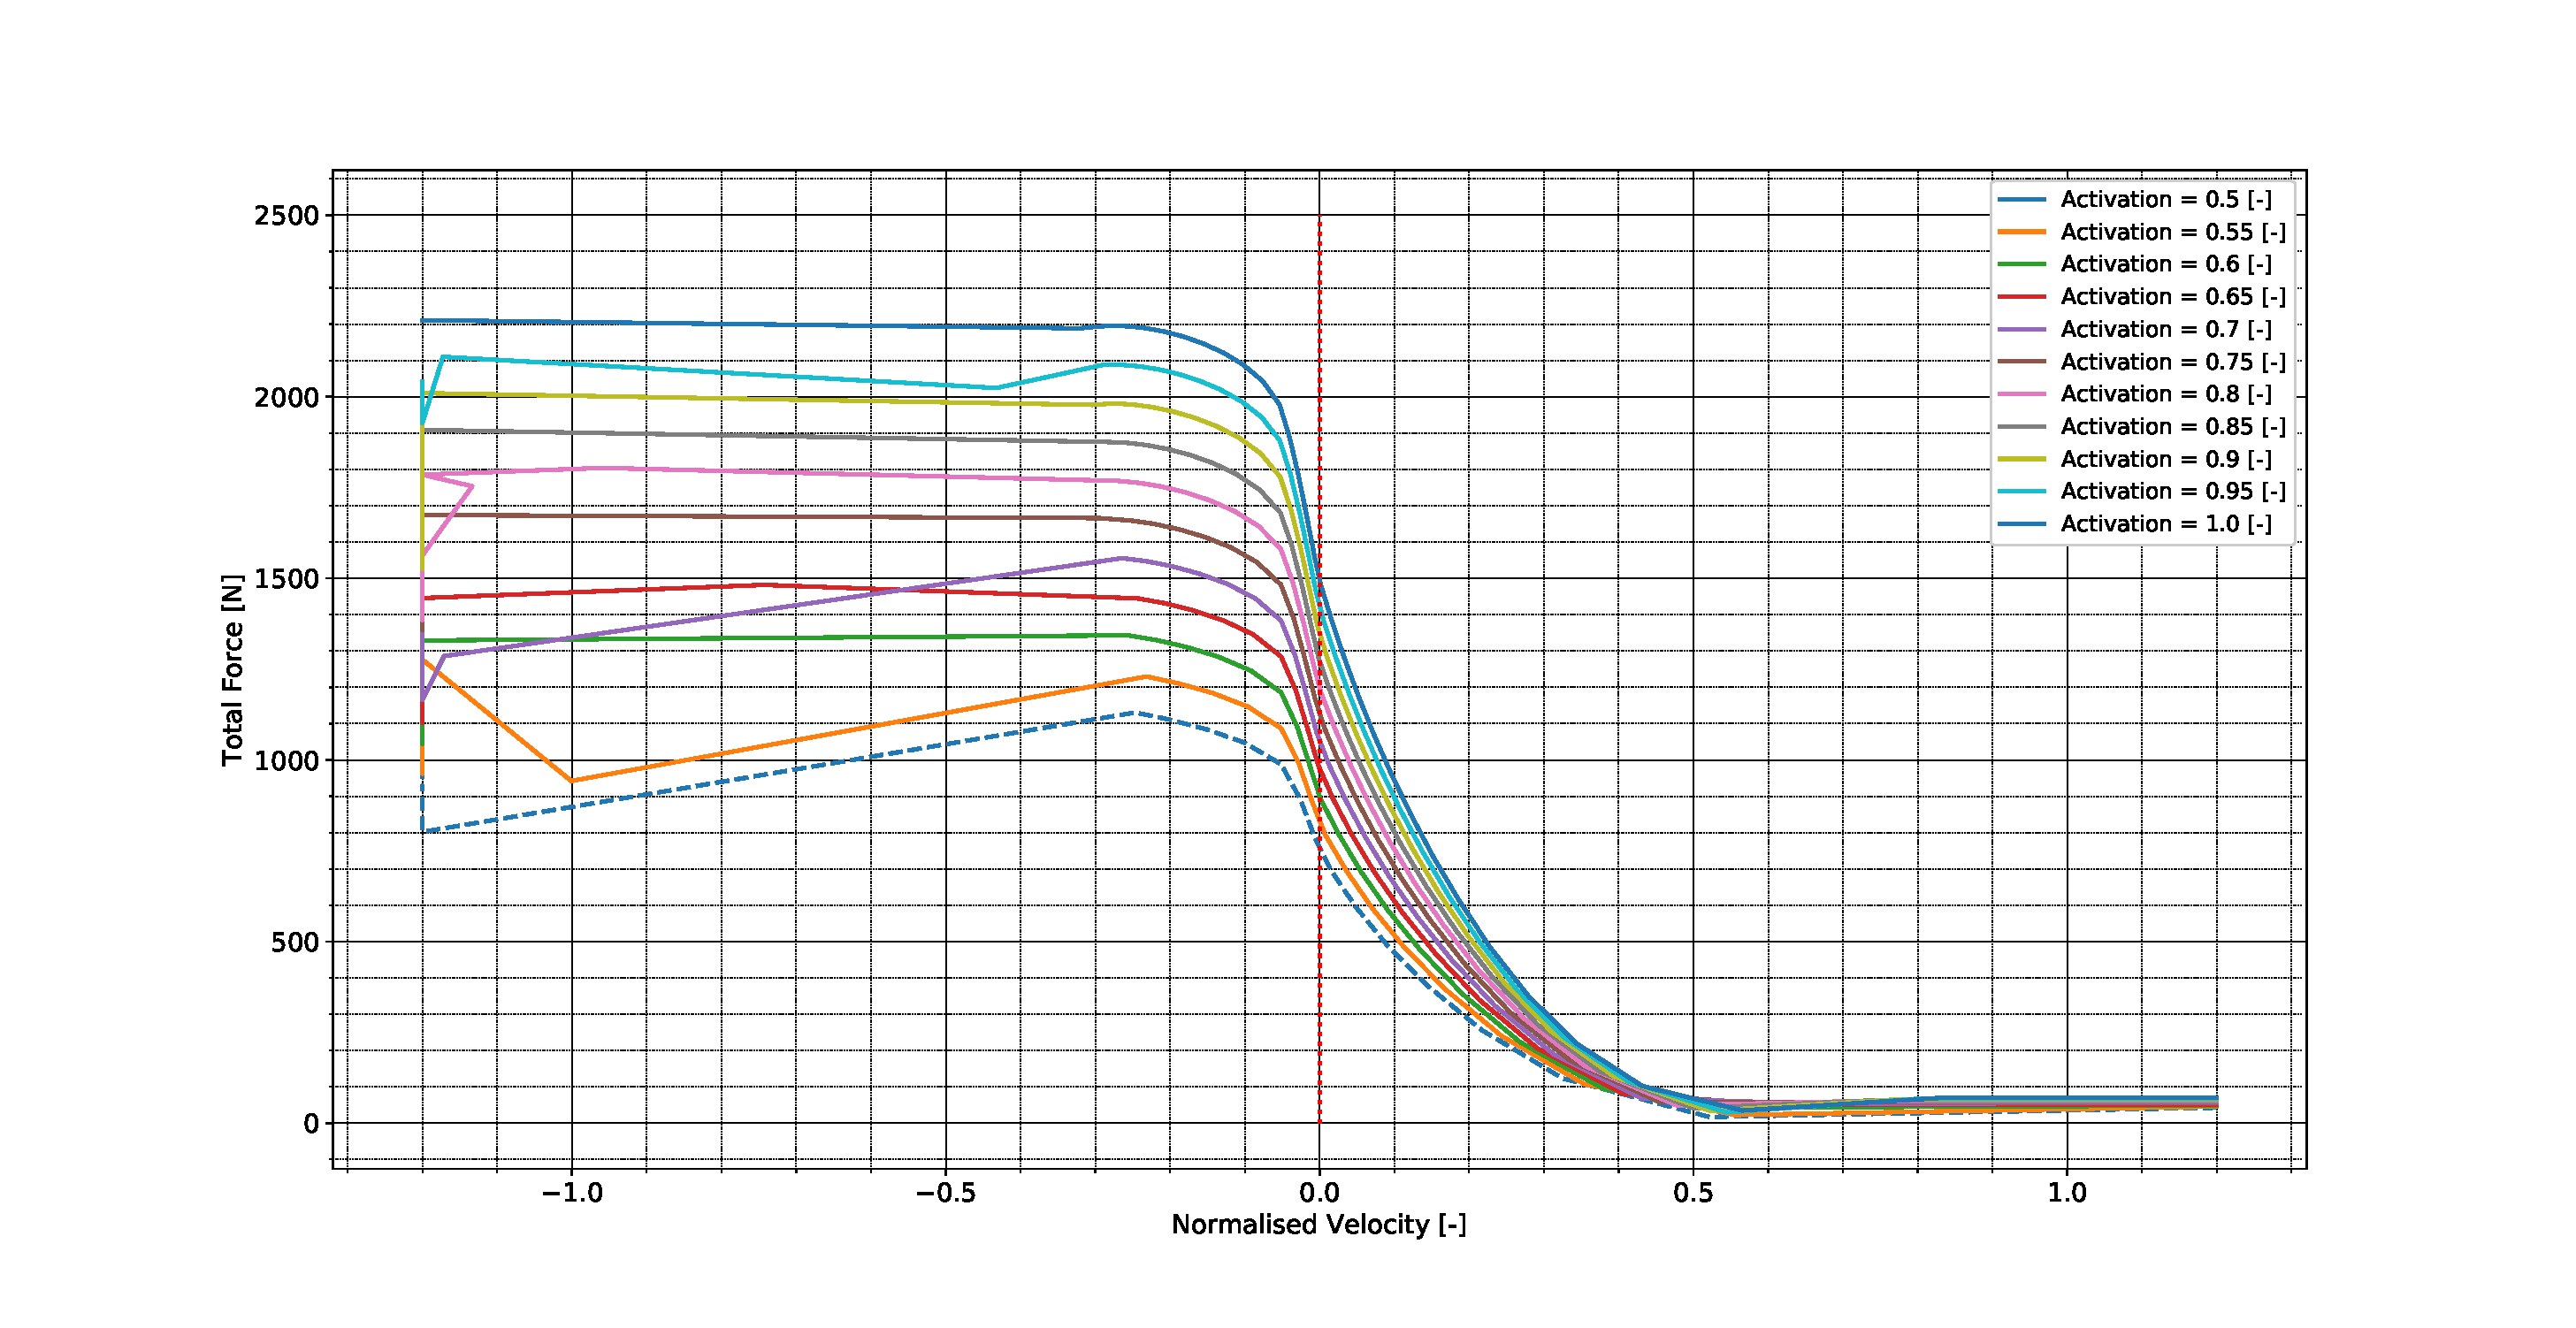
\includegraphics[width=0.8\textwidth]{2f.eps}
\caption{Plot of the relationship between total force (active + passive) and velocity with varying activation from 0.5 to 1.0, with steps of 0.05. A velocity of 0.0 corresponds to the isometric case. The external load applied to the muscle ranges from 1 to 321 kg, with steps of 10. By means of visualization, the activation value $a=0.5$ has been represented by a dashed line, such as in Figure \ref{figure:2b}}
\label{figure:2df}
\end{figure}

Following what has been stated in point 2.e, Figure \ref{figure:2df} shows that increasing the activation -- which increases the maximum active force that the muscle is able to generate, as seen in Figure \ref{figure:2b} -- increases the force that the muscle exhibits at the isometric point. On the right-hand side, less differences are observed in the muscle's behaviour when we vary the activation, since the same passive resistance mechanism is at work, independently of the activation.
When varying the activation, the isometric forces in Figure \ref{figure:2df} are similar to the maximum active forces shown in Figure \ref{figure:2b}.

\end{document}

%%% Local Variables:
%%% mode: latex
%%% TeX-master: t
%%% End: